\documentclass[11pt]{article}

    \usepackage[breakable]{tcolorbox}
    \usepackage{parskip} % Stop auto-indenting (to mimic markdown behaviour)
    
    \usepackage{iftex}
    \ifPDFTeX
    	\usepackage[T1]{fontenc}
    	\usepackage{mathpazo}
    \else
    	\usepackage{fontspec}
    \fi

    % Basic figure setup, for now with no caption control since it's done
    % automatically by Pandoc (which extracts ![](path) syntax from Markdown).
    \usepackage{graphicx}
    % Maintain compatibility with old templates. Remove in nbconvert 6.0
    \let\Oldincludegraphics\includegraphics
    % Ensure that by default, figures have no caption (until we provide a
    % proper Figure object with a Caption API and a way to capture that
    % in the conversion process - todo).
    \usepackage{caption}
    \usepackage{subcaption}
    % \DeclareCaptionFormat{nocaption}{}
    % \captionsetup{format=nocaption,aboveskip=0pt,belowskip=0pt}

    \usepackage{float}
    \floatplacement{figure}{H} % forces figures to be placed at the correct location
    \usepackage{xcolor} % Allow colors to be defined
    \usepackage{enumerate} % Needed for markdown enumerations to work
    \usepackage{geometry} % Used to adjust the document margins
    \usepackage{amsmath} % Equations
    \usepackage{amssymb} % Equations
    \usepackage{textcomp} % defines textquotesingle
    % Hack from http://tex.stackexchange.com/a/47451/13684:
    \AtBeginDocument{%
        \def\PYZsq{\textquotesingle}% Upright quotes in Pygmentized code
    }
    \usepackage{upquote} % Upright quotes for verbatim code
    \usepackage{eurosym} % defines \euro
    \usepackage[mathletters]{ucs} % Extended unicode (utf-8) support
    \usepackage{fancyvrb} % verbatim replacement that allows latex
    \usepackage{grffile} % extends the file name processing of package graphics 
                         % to support a larger range
    \makeatletter % fix for old versions of grffile with XeLaTeX
    \@ifpackagelater{grffile}{2019/11/01}
    {
      % Do nothing on new versions
    }
    {
      \def\Gread@@xetex#1{%
        \IfFileExists{"\Gin@base".bb}%
        {\Gread@eps{\Gin@base.bb}}%
        {\Gread@@xetex@aux#1}%
      }
    }
    \makeatother
    \usepackage[Export]{adjustbox} % Used to constrain images to a maximum size
    \adjustboxset{max size={0.9\linewidth}{0.9\paperheight}}

    % The hyperref package gives us a pdf with properly built
    % internal navigation ('pdf bookmarks' for the table of contents,
    % internal cross-reference links, web links for URLs, etc.)
    \usepackage{hyperref}
    % The default LaTeX title has an obnoxious amount of whitespace. By default,
    % titling removes some of it. It also provides customization options.
    \usepackage{titling}
    \usepackage{longtable} % longtable support required by pandoc >1.10
    \usepackage{booktabs}  % table support for pandoc > 1.12.2
    \usepackage[inline]{enumitem} % IRkernel/repr support (it uses the enumerate* environment)
    \usepackage[normalem]{ulem} % ulem is needed to support strikethroughs (\sout)
                                % normalem makes italics be italics, not underlines
    \usepackage{mathrsfs}
    \usepackage{tabularx}

    
    % Colors for the hyperref package
    \definecolor{urlcolor}{rgb}{0,.145,.698}
    \definecolor{linkcolor}{rgb}{.71,0.21,0.01}
    \definecolor{citecolor}{rgb}{.12,.54,.11}

    % ANSI colors
    \definecolor{ansi-black}{HTML}{3E424D}
    \definecolor{ansi-black-intense}{HTML}{282C36}
    \definecolor{ansi-red}{HTML}{E75C58}
    \definecolor{ansi-red-intense}{HTML}{B22B31}
    \definecolor{ansi-green}{HTML}{00A250}
    \definecolor{ansi-green-intense}{HTML}{007427}
    \definecolor{ansi-yellow}{HTML}{DDB62B}
    \definecolor{ansi-yellow-intense}{HTML}{B27D12}
    \definecolor{ansi-blue}{HTML}{208FFB}
    \definecolor{ansi-blue-intense}{HTML}{0065CA}
    \definecolor{ansi-magenta}{HTML}{D160C4}
    \definecolor{ansi-magenta-intense}{HTML}{A03196}
    \definecolor{ansi-cyan}{HTML}{60C6C8}
    \definecolor{ansi-cyan-intense}{HTML}{258F8F}
    \definecolor{ansi-white}{HTML}{C5C1B4}
    \definecolor{ansi-white-intense}{HTML}{A1A6B2}
    \definecolor{ansi-default-inverse-fg}{HTML}{FFFFFF}
    \definecolor{ansi-default-inverse-bg}{HTML}{000000}

    % common color for the border for error outputs.
    \definecolor{outerrorbackground}{HTML}{FFDFDF}

    % commands and environments needed by pandoc snippets
    % extracted from the output of `pandoc -s`
    \providecommand{\tightlist}{%
      \setlength{\itemsep}{0pt}\setlength{\parskip}{0pt}}
    \DefineVerbatimEnvironment{Highlighting}{Verbatim}{commandchars=\\\{\}}
    % Add ',fontsize=\small' for more characters per line
    \newenvironment{Shaded}{}{}
    \newcommand{\KeywordTok}[1]{\textcolor[rgb]{0.00,0.44,0.13}{\textbf{{#1}}}}
    \newcommand{\DataTypeTok}[1]{\textcolor[rgb]{0.56,0.13,0.00}{{#1}}}
    \newcommand{\DecValTok}[1]{\textcolor[rgb]{0.25,0.63,0.44}{{#1}}}
    \newcommand{\BaseNTok}[1]{\textcolor[rgb]{0.25,0.63,0.44}{{#1}}}
    \newcommand{\FloatTok}[1]{\textcolor[rgb]{0.25,0.63,0.44}{{#1}}}
    \newcommand{\CharTok}[1]{\textcolor[rgb]{0.25,0.44,0.63}{{#1}}}
    \newcommand{\StringTok}[1]{\textcolor[rgb]{0.25,0.44,0.63}{{#1}}}
    \newcommand{\CommentTok}[1]{\textcolor[rgb]{0.38,0.63,0.69}{\textit{{#1}}}}
    \newcommand{\OtherTok}[1]{\textcolor[rgb]{0.00,0.44,0.13}{{#1}}}
    \newcommand{\AlertTok}[1]{\textcolor[rgb]{1.00,0.00,0.00}{\textbf{{#1}}}}
    \newcommand{\FunctionTok}[1]{\textcolor[rgb]{0.02,0.16,0.49}{{#1}}}
    \newcommand{\RegionMarkerTok}[1]{{#1}}
    \newcommand{\ErrorTok}[1]{\textcolor[rgb]{1.00,0.00,0.00}{\textbf{{#1}}}}
    \newcommand{\NormalTok}[1]{{#1}}
    
    % Additional commands for more recent versions of Pandoc
    \newcommand{\ConstantTok}[1]{\textcolor[rgb]{0.53,0.00,0.00}{{#1}}}
    \newcommand{\SpecialCharTok}[1]{\textcolor[rgb]{0.25,0.44,0.63}{{#1}}}
    \newcommand{\VerbatimStringTok}[1]{\textcolor[rgb]{0.25,0.44,0.63}{{#1}}}
    \newcommand{\SpecialStringTok}[1]{\textcolor[rgb]{0.73,0.40,0.53}{{#1}}}
    \newcommand{\ImportTok}[1]{{#1}}
    \newcommand{\DocumentationTok}[1]{\textcolor[rgb]{0.73,0.13,0.13}{\textit{{#1}}}}
    \newcommand{\AnnotationTok}[1]{\textcolor[rgb]{0.38,0.63,0.69}{\textbf{\textit{{#1}}}}}
    \newcommand{\CommentVarTok}[1]{\textcolor[rgb]{0.38,0.63,0.69}{\textbf{\textit{{#1}}}}}
    \newcommand{\VariableTok}[1]{\textcolor[rgb]{0.10,0.09,0.49}{{#1}}}
    \newcommand{\ControlFlowTok}[1]{\textcolor[rgb]{0.00,0.44,0.13}{\textbf{{#1}}}}
    \newcommand{\OperatorTok}[1]{\textcolor[rgb]{0.40,0.40,0.40}{{#1}}}
    \newcommand{\BuiltInTok}[1]{{#1}}
    \newcommand{\ExtensionTok}[1]{{#1}}
    \newcommand{\PreprocessorTok}[1]{\textcolor[rgb]{0.74,0.48,0.00}{{#1}}}
    \newcommand{\AttributeTok}[1]{\textcolor[rgb]{0.49,0.56,0.16}{{#1}}}
    \newcommand{\InformationTok}[1]{\textcolor[rgb]{0.38,0.63,0.69}{\textbf{\textit{{#1}}}}}
    \newcommand{\WarningTok}[1]{\textcolor[rgb]{0.38,0.63,0.69}{\textbf{\textit{{#1}}}}}
    
    
    % Define a nice break command that doesn't care if a line doesn't already
    % exist.
    \def\br{\hspace*{\fill} \\* }
    % Math Jax compatibility definitions
    \def\gt{>}
    \def\lt{<}
    \let\Oldtex\TeX
    \let\Oldlatex\LaTeX
    \renewcommand{\TeX}{\textrm{\Oldtex}}
    \renewcommand{\LaTeX}{\textrm{\Oldlatex}}
    % Document parameters
    % Document title
    \title{Hanami and Ramen}
    \date{}
    
% Pygments definitions
\makeatletter
\def\PY@reset{\let\PY@it=\relax \let\PY@bf=\relax%
    \let\PY@ul=\relax \let\PY@tc=\relax%
    \let\PY@bc=\relax \let\PY@ff=\relax}
\def\PY@tok#1{\csname PY@tok@#1\endcsname}
\def\PY@toks#1+{\ifx\relax#1\empty\else%
    \PY@tok{#1}\expandafter\PY@toks\fi}
\def\PY@do#1{\PY@bc{\PY@tc{\PY@ul{%
    \PY@it{\PY@bf{\PY@ff{#1}}}}}}}
\def\PY#1#2{\PY@reset\PY@toks#1+\relax+\PY@do{#2}}

\@namedef{PY@tok@w}{\def\PY@tc##1{\textcolor[rgb]{0.73,0.73,0.73}{##1}}}
\@namedef{PY@tok@c}{\let\PY@it=\textit\def\PY@tc##1{\textcolor[rgb]{0.25,0.50,0.50}{##1}}}
\@namedef{PY@tok@cp}{\def\PY@tc##1{\textcolor[rgb]{0.74,0.48,0.00}{##1}}}
\@namedef{PY@tok@k}{\let\PY@bf=\textbf\def\PY@tc##1{\textcolor[rgb]{0.00,0.50,0.00}{##1}}}
\@namedef{PY@tok@kp}{\def\PY@tc##1{\textcolor[rgb]{0.00,0.50,0.00}{##1}}}
\@namedef{PY@tok@kt}{\def\PY@tc##1{\textcolor[rgb]{0.69,0.00,0.25}{##1}}}
\@namedef{PY@tok@o}{\def\PY@tc##1{\textcolor[rgb]{0.40,0.40,0.40}{##1}}}
\@namedef{PY@tok@ow}{\let\PY@bf=\textbf\def\PY@tc##1{\textcolor[rgb]{0.67,0.13,1.00}{##1}}}
\@namedef{PY@tok@nb}{\def\PY@tc##1{\textcolor[rgb]{0.00,0.50,0.00}{##1}}}
\@namedef{PY@tok@nf}{\def\PY@tc##1{\textcolor[rgb]{0.00,0.00,1.00}{##1}}}
\@namedef{PY@tok@nc}{\let\PY@bf=\textbf\def\PY@tc##1{\textcolor[rgb]{0.00,0.00,1.00}{##1}}}
\@namedef{PY@tok@nn}{\let\PY@bf=\textbf\def\PY@tc##1{\textcolor[rgb]{0.00,0.00,1.00}{##1}}}
\@namedef{PY@tok@ne}{\let\PY@bf=\textbf\def\PY@tc##1{\textcolor[rgb]{0.82,0.25,0.23}{##1}}}
\@namedef{PY@tok@nv}{\def\PY@tc##1{\textcolor[rgb]{0.10,0.09,0.49}{##1}}}
\@namedef{PY@tok@no}{\def\PY@tc##1{\textcolor[rgb]{0.53,0.00,0.00}{##1}}}
\@namedef{PY@tok@nl}{\def\PY@tc##1{\textcolor[rgb]{0.63,0.63,0.00}{##1}}}
\@namedef{PY@tok@ni}{\let\PY@bf=\textbf\def\PY@tc##1{\textcolor[rgb]{0.60,0.60,0.60}{##1}}}
\@namedef{PY@tok@na}{\def\PY@tc##1{\textcolor[rgb]{0.49,0.56,0.16}{##1}}}
\@namedef{PY@tok@nt}{\let\PY@bf=\textbf\def\PY@tc##1{\textcolor[rgb]{0.00,0.50,0.00}{##1}}}
\@namedef{PY@tok@nd}{\def\PY@tc##1{\textcolor[rgb]{0.67,0.13,1.00}{##1}}}
\@namedef{PY@tok@s}{\def\PY@tc##1{\textcolor[rgb]{0.73,0.13,0.13}{##1}}}
\@namedef{PY@tok@sd}{\let\PY@it=\textit\def\PY@tc##1{\textcolor[rgb]{0.73,0.13,0.13}{##1}}}
\@namedef{PY@tok@si}{\let\PY@bf=\textbf\def\PY@tc##1{\textcolor[rgb]{0.73,0.40,0.53}{##1}}}
\@namedef{PY@tok@se}{\let\PY@bf=\textbf\def\PY@tc##1{\textcolor[rgb]{0.73,0.40,0.13}{##1}}}
\@namedef{PY@tok@sr}{\def\PY@tc##1{\textcolor[rgb]{0.73,0.40,0.53}{##1}}}
\@namedef{PY@tok@ss}{\def\PY@tc##1{\textcolor[rgb]{0.10,0.09,0.49}{##1}}}
\@namedef{PY@tok@sx}{\def\PY@tc##1{\textcolor[rgb]{0.00,0.50,0.00}{##1}}}
\@namedef{PY@tok@m}{\def\PY@tc##1{\textcolor[rgb]{0.40,0.40,0.40}{##1}}}
\@namedef{PY@tok@gh}{\let\PY@bf=\textbf\def\PY@tc##1{\textcolor[rgb]{0.00,0.00,0.50}{##1}}}
\@namedef{PY@tok@gu}{\let\PY@bf=\textbf\def\PY@tc##1{\textcolor[rgb]{0.50,0.00,0.50}{##1}}}
\@namedef{PY@tok@gd}{\def\PY@tc##1{\textcolor[rgb]{0.63,0.00,0.00}{##1}}}
\@namedef{PY@tok@gi}{\def\PY@tc##1{\textcolor[rgb]{0.00,0.63,0.00}{##1}}}
\@namedef{PY@tok@gr}{\def\PY@tc##1{\textcolor[rgb]{1.00,0.00,0.00}{##1}}}
\@namedef{PY@tok@ge}{\let\PY@it=\textit}
\@namedef{PY@tok@gs}{\let\PY@bf=\textbf}
\@namedef{PY@tok@gp}{\let\PY@bf=\textbf\def\PY@tc##1{\textcolor[rgb]{0.00,0.00,0.50}{##1}}}
\@namedef{PY@tok@go}{\def\PY@tc##1{\textcolor[rgb]{0.53,0.53,0.53}{##1}}}
\@namedef{PY@tok@gt}{\def\PY@tc##1{\textcolor[rgb]{0.00,0.27,0.87}{##1}}}
\@namedef{PY@tok@err}{\def\PY@bc##1{{\setlength{\fboxsep}{\string -\fboxrule}\fcolorbox[rgb]{1.00,0.00,0.00}{1,1,1}{\strut ##1}}}}
\@namedef{PY@tok@kc}{\let\PY@bf=\textbf\def\PY@tc##1{\textcolor[rgb]{0.00,0.50,0.00}{##1}}}
\@namedef{PY@tok@kd}{\let\PY@bf=\textbf\def\PY@tc##1{\textcolor[rgb]{0.00,0.50,0.00}{##1}}}
\@namedef{PY@tok@kn}{\let\PY@bf=\textbf\def\PY@tc##1{\textcolor[rgb]{0.00,0.50,0.00}{##1}}}
\@namedef{PY@tok@kr}{\let\PY@bf=\textbf\def\PY@tc##1{\textcolor[rgb]{0.00,0.50,0.00}{##1}}}
\@namedef{PY@tok@bp}{\def\PY@tc##1{\textcolor[rgb]{0.00,0.50,0.00}{##1}}}
\@namedef{PY@tok@fm}{\def\PY@tc##1{\textcolor[rgb]{0.00,0.00,1.00}{##1}}}
\@namedef{PY@tok@vc}{\def\PY@tc##1{\textcolor[rgb]{0.10,0.09,0.49}{##1}}}
\@namedef{PY@tok@vg}{\def\PY@tc##1{\textcolor[rgb]{0.10,0.09,0.49}{##1}}}
\@namedef{PY@tok@vi}{\def\PY@tc##1{\textcolor[rgb]{0.10,0.09,0.49}{##1}}}
\@namedef{PY@tok@vm}{\def\PY@tc##1{\textcolor[rgb]{0.10,0.09,0.49}{##1}}}
\@namedef{PY@tok@sa}{\def\PY@tc##1{\textcolor[rgb]{0.73,0.13,0.13}{##1}}}
\@namedef{PY@tok@sb}{\def\PY@tc##1{\textcolor[rgb]{0.73,0.13,0.13}{##1}}}
\@namedef{PY@tok@sc}{\def\PY@tc##1{\textcolor[rgb]{0.73,0.13,0.13}{##1}}}
\@namedef{PY@tok@dl}{\def\PY@tc##1{\textcolor[rgb]{0.73,0.13,0.13}{##1}}}
\@namedef{PY@tok@s2}{\def\PY@tc##1{\textcolor[rgb]{0.73,0.13,0.13}{##1}}}
\@namedef{PY@tok@sh}{\def\PY@tc##1{\textcolor[rgb]{0.73,0.13,0.13}{##1}}}
\@namedef{PY@tok@s1}{\def\PY@tc##1{\textcolor[rgb]{0.73,0.13,0.13}{##1}}}
\@namedef{PY@tok@mb}{\def\PY@tc##1{\textcolor[rgb]{0.40,0.40,0.40}{##1}}}
\@namedef{PY@tok@mf}{\def\PY@tc##1{\textcolor[rgb]{0.40,0.40,0.40}{##1}}}
\@namedef{PY@tok@mh}{\def\PY@tc##1{\textcolor[rgb]{0.40,0.40,0.40}{##1}}}
\@namedef{PY@tok@mi}{\def\PY@tc##1{\textcolor[rgb]{0.40,0.40,0.40}{##1}}}
\@namedef{PY@tok@il}{\def\PY@tc##1{\textcolor[rgb]{0.40,0.40,0.40}{##1}}}
\@namedef{PY@tok@mo}{\def\PY@tc##1{\textcolor[rgb]{0.40,0.40,0.40}{##1}}}
\@namedef{PY@tok@ch}{\let\PY@it=\textit\def\PY@tc##1{\textcolor[rgb]{0.25,0.50,0.50}{##1}}}
\@namedef{PY@tok@cm}{\let\PY@it=\textit\def\PY@tc##1{\textcolor[rgb]{0.25,0.50,0.50}{##1}}}
\@namedef{PY@tok@cpf}{\let\PY@it=\textit\def\PY@tc##1{\textcolor[rgb]{0.25,0.50,0.50}{##1}}}
\@namedef{PY@tok@c1}{\let\PY@it=\textit\def\PY@tc##1{\textcolor[rgb]{0.25,0.50,0.50}{##1}}}
\@namedef{PY@tok@cs}{\let\PY@it=\textit\def\PY@tc##1{\textcolor[rgb]{0.25,0.50,0.50}{##1}}}

\def\PYZbs{\char`\\}
\def\PYZus{\char`\_}
\def\PYZob{\char`\{}
\def\PYZcb{\char`\}}
\def\PYZca{\char`\^}
\def\PYZam{\char`\&}
\def\PYZlt{\char`\<}
\def\PYZgt{\char`\>}
\def\PYZsh{\char`\#}
\def\PYZpc{\char`\%}
\def\PYZdl{\char`\$}
\def\PYZhy{\char`\-}
\def\PYZsq{\char`\'}
\def\PYZdq{\char`\"}
\def\PYZti{\char`\~}
% for compatibility with earlier versions
\def\PYZat{@}
\def\PYZlb{[}
\def\PYZrb{]}
\makeatother


    % For linebreaks inside Verbatim environment from package fancyvrb. 
    \makeatletter
        \newbox\Wrappedcontinuationbox 
        \newbox\Wrappedvisiblespacebox 
        \newcommand*\Wrappedvisiblespace {\textcolor{red}{\textvisiblespace}} 
        \newcommand*\Wrappedcontinuationsymbol {\textcolor{red}{\llap{\tiny$\m@th\hookrightarrow$}}} 
        \newcommand*\Wrappedcontinuationindent {3ex } 
        \newcommand*\Wrappedafterbreak {\kern\Wrappedcontinuationindent\copy\Wrappedcontinuationbox} 
        % Take advantage of the already applied Pygments mark-up to insert 
        % potential linebreaks for TeX processing. 
        %        {, <, #, %, $, ' and ": go to next line. 
        %        _, }, ^, &, >, - and ~: stay at end of broken line. 
        % Use of \textquotesingle for straight quote. 
        \newcommand*\Wrappedbreaksatspecials {% 
            \def\PYGZus{\discretionary{\char`\_}{\Wrappedafterbreak}{\char`\_}}% 
            \def\PYGZob{\discretionary{}{\Wrappedafterbreak\char`\{}{\char`\{}}% 
            \def\PYGZcb{\discretionary{\char`\}}{\Wrappedafterbreak}{\char`\}}}% 
            \def\PYGZca{\discretionary{\char`\^}{\Wrappedafterbreak}{\char`\^}}% 
            \def\PYGZam{\discretionary{\char`\&}{\Wrappedafterbreak}{\char`\&}}% 
            \def\PYGZlt{\discretionary{}{\Wrappedafterbreak\char`\<}{\char`\<}}% 
            \def\PYGZgt{\discretionary{\char`\>}{\Wrappedafterbreak}{\char`\>}}% 
            \def\PYGZsh{\discretionary{}{\Wrappedafterbreak\char`\#}{\char`\#}}% 
            \def\PYGZpc{\discretionary{}{\Wrappedafterbreak\char`\%}{\char`\%}}% 
            \def\PYGZdl{\discretionary{}{\Wrappedafterbreak\char`\$}{\char`\$}}% 
            \def\PYGZhy{\discretionary{\char`\-}{\Wrappedafterbreak}{\char`\-}}% 
            \def\PYGZsq{\discretionary{}{\Wrappedafterbreak\textquotesingle}{\textquotesingle}}% 
            \def\PYGZdq{\discretionary{}{\Wrappedafterbreak\char`\"}{\char`\"}}% 
            \def\PYGZti{\discretionary{\char`\~}{\Wrappedafterbreak}{\char`\~}}% 
        } 
        % Some characters . , ; ? ! / are not pygmentized. 
        % This macro makes them "active" and they will insert potential linebreaks 
        \newcommand*\Wrappedbreaksatpunct {% 
            \lccode`\~`\.\lowercase{\def~}{\discretionary{\hbox{\char`\.}}{\Wrappedafterbreak}{\hbox{\char`\.}}}% 
            \lccode`\~`\,\lowercase{\def~}{\discretionary{\hbox{\char`\,}}{\Wrappedafterbreak}{\hbox{\char`\,}}}% 
            \lccode`\~`\;\lowercase{\def~}{\discretionary{\hbox{\char`\;}}{\Wrappedafterbreak}{\hbox{\char`\;}}}% 
            \lccode`\~`\:\lowercase{\def~}{\discretionary{\hbox{\char`\:}}{\Wrappedafterbreak}{\hbox{\char`\:}}}% 
            \lccode`\~`\?\lowercase{\def~}{\discretionary{\hbox{\char`\?}}{\Wrappedafterbreak}{\hbox{\char`\?}}}% 
            \lccode`\~`\!\lowercase{\def~}{\discretionary{\hbox{\char`\!}}{\Wrappedafterbreak}{\hbox{\char`\!}}}% 
            \lccode`\~`\/\lowercase{\def~}{\discretionary{\hbox{\char`\/}}{\Wrappedafterbreak}{\hbox{\char`\/}}}% 
            \catcode`\.\active
            \catcode`\,\active 
            \catcode`\;\active
            \catcode`\:\active
            \catcode`\?\active
            \catcode`\!\active
            \catcode`\/\active 
            \lccode`\~`\~ 	
        }
    \makeatother

    \let\OriginalVerbatim=\Verbatim
    \makeatletter
    \renewcommand{\Verbatim}[1][1]{%
        %\parskip\z@skip
        \sbox\Wrappedcontinuationbox {\Wrappedcontinuationsymbol}%
        \sbox\Wrappedvisiblespacebox {\FV@SetupFont\Wrappedvisiblespace}%
        \def\FancyVerbFormatLine ##1{\hsize\linewidth
            \vtop{\raggedright\hyphenpenalty\z@\exhyphenpenalty\z@
                \doublehyphendemerits\z@\finalhyphendemerits\z@
                \strut ##1\strut}%
        }%
        % If the linebreak is at a space, the latter will be displayed as visible
        % space at end of first line, and a continuation symbol starts next line.
        % Stretch/shrink are however usually zero for typewriter font.
        \def\FV@Space {%
            \nobreak\hskip\z@ plus\fontdimen3\font minus\fontdimen4\font
            \discretionary{\copy\Wrappedvisiblespacebox}{\Wrappedafterbreak}
            {\kern\fontdimen2\font}%
        }%
        
        % Allow breaks at special characters using \PYG... macros.
        \Wrappedbreaksatspecials
        % Breaks at punctuation characters . , ; ? ! and / need catcode=\active 	
        \OriginalVerbatim[#1,codes*=\Wrappedbreaksatpunct]%
    }
    \makeatother

    % Exact colors from NB
    \definecolor{incolor}{HTML}{303F9F}
    \definecolor{outcolor}{HTML}{D84315}
    \definecolor{cellborder}{HTML}{CFCFCF}
    \definecolor{cellbackground}{HTML}{F7F7F7}
    
    % prompt
    \makeatletter
    \newcommand{\boxspacing}{\kern\kvtcb@left@rule\kern\kvtcb@boxsep}
    \makeatother
    \newcommand{\prompt}[4]{
        {\ttfamily\llap{{\color{#2}[#3]:\hspace{3pt}#4}}\vspace{-\baselineskip}}
    }
    

    
    % Prevent overflowing lines due to hard-to-break entities
    \sloppy 
    % Setup hyperref package
    \hypersetup{
      breaklinks=true,  % so long urls are correctly broken across lines
      colorlinks=true,
      urlcolor=urlcolor,
      linkcolor=linkcolor,
      citecolor=citecolor,
      }
    % Slightly bigger margins than the latex defaults
    
    \geometry{verbose,tmargin=1in,bmargin=1in,lmargin=1in,rmargin=1in}
    
    

\begin{document}
    
\maketitle

    \hypertarget{introduction}{%
\section{Introduction}\label{introduction}}

    Hanami (``flower viewing'') is the traditional custom of viewing and
enjoying the beauty of flowers (mainly cherry blossoms) and springtime
in Japan. Each year the \emph{cherry blossom front}, the advance of
blooming of cherry blossoms across Japan, is tracked as it slowly moves
northward. The front generally indicates the opening of the first
blossoms (kaika) rather than the arrival of full bloom (mankai).
Forecasts for the cherry blossom front by are closely followed by those
who wish to enjoy hanami as the blossoms only last for one to two weeks.

To enjoy Hanami, one can admire from a distance in which the cherry
blossoms have been described as appearing as beautiful clouds or have a
picnic under the blooming trees. But why not enjoy a nice stroll in a park after
enjoying a nice meal such as a bowl of Ramen. Here is a little info on Ramen.

While the exact origins of ramen noodles is up to debate (Japan or China
origin), what is not up for debate is how Ramen shops across Japan have
really made Ramen their own. As the name suggest, Ramen shops specialize
in ramen dishes. Ramen in simple terms are wheat-flour noodles served in
broth. But Ramen is anything but simple. With over more than 10,000
ramen shops in Japan, each shop provides a different take on the dish of
Ramen.

The goal of this project is to try to find the best locations/spots in Japan in
which to enjoy both Hanami and Ramen from \textbf{April 15th to May
15th}. Best in this instance, refers to \textbf{promixity to train station}, 
\textbf{recommendation}, and \textbf{Ramen shops} located nearby.

Note: Hanami Spots and Viewing Spots are used interchangeably throughout
the project.

\hypertarget{data}{%
\section{Data}\label{data}}

    With the criteria mention in the Introduction, factors that influenced our decision were:
\begin{itemize}
  \tightlist
  \item Timing of cherry blossoming in cities across Japan 
  \item Proximity to a train station 
  \item Recommended Cherry Blossom viewing spots (Hanami) spots 
  \item Ramen shops located close to Hanami spots
  \end{itemize}

Following data sources were used to extract/generate the required
information: 

\begin{itemize}
  \tightlist
  \item Average Cherry Blossoms blooming dates using data gathered from: \url{https://www.japan-guide.com/e/e2011_when.html}. 
  \item Recommended Cherry Blossom viewing spots gathered from: \url{https://www.japan-guide.com/e/e2011_where.html} 
  \item \textbf{Google Places API} was used to obtain the coordinates of each recommended viewing spot. The coordinates were used 
  to obtain the region for each of the recommended viewing spots by use of information found on Wikipedia. 
  \item Ramen shops and Train stations around each recommended Hanami spot were obtained using the \textbf{Foursquare API}
\end{itemize}

With the data collected, locations  were narrowed down based off the criteria mentioned above.

    \hypertarget{average-cherry-blossoms-blooming-dates}{%
\subsection{Average Cherry Blossoms blooming
dates}\label{average-cherry-blossoms-blooming-dates}}

The typical timing for the blooming of cherry blossoms in cities across Japan was obtained.

This information was found from the following source \url{https://www.japan-guide.com/e/e2011_when.html}.

The data is contained within a table on the webpage, meaning the data can be read directly into a pandas dataframe.

Only the cities which are typically in full bloom from April 15th to May
15th were stored within the \texttt{averageBlooming\_df} dataframe.

\begin{table}[h]
\small
\centering
\caption{\texttt{averageBlooming\_df}: Cities Blooming dates between April 15th to May 15th}
\begin{tabular}{ccc}
\toprule
CITY      & AVERAGE\_OPENING & AVERAGE\_FULL\_BLOOM \\
\midrule
  Sapporo &    May 3        &    May 7           \\
 Hakodate & April 30        &    May 4           \\
 Hirosaki & April 23        & April 28           \\
   Sendai & April 11        & April 16           \\
Matsumoto & April 10        & April 15           \\
 Takayama & April 15        & April 20           \\
\bottomrule
\end{tabular}
\end{table}


    \hypertarget{cherry-blossom-viewing-spots}{%
\subsection{Cherry Blossom Viewing
Spots}\label{cherry-blossom-viewing-spots}}

Recommendations for the best cherry blossom viewing spots (Hanami Spots) can be found at \url{https://www.japan-guide.com/e/e2011_where.html}.

The information for the different recommended Cherry Blossom Viewing Spots were scraped and loaded into a panadas dataframe, \texttt{viewingSpot\_df}.
The information of interest collected for each recommended viewing spot was:

\begin{itemize}
\tightlist
  \item City
  \item Viewing Spot Name
  \item Description
  \item Ratings
  \item Ratings Description
\end{itemize}

A total  of 48 recommended viewing spots across Japan are listed on the site. On inspection, the information for each recommended viewing spot 
seemed to be incomplete. Some data cleaning was conducted and will be discussed in the following subsections.

    \hypertarget{obtaining-geographical-information-for-the-recommended-viewing-spots}{%
\subsubsection{Obtaining geographical information for the recommended Viewing Spots}\label{obtaining-geographical-information-for-the-recommended-viewing-spots}}

The \texttt{CITY} column in \texttt{viewingSpot\_df} contained some values which aren't exactly cities.

Reverse geocoding through the use of the Google Places API was used to obtain the geographical information for
each of the viewing spots to determine the city, prefecture, and coordinates for each of the viewing spots.

    \hypertarget{finding-the-region-for-each-of-the-locations-within-viewingspot_df.}{%
\subsubsection{Finding the region for each of the locations within viewingSpot\_df.}\label{finding-the-region-for-each-of-the-locations-within-viewingspot_df}}

The geographical information for each of the recommended viewing spots was used to find the region in which each location are within. 
This was accomplished by accessing a table located at \href{https://simple.wikipedia.org/wiki/Prefectures_of_Japan}{Wikipedia},
which lists each prefecture with corresponding region.

The final thing to do was to only concentrate on those recommended viewing spots located within one of the cities found within the 
\texttt{averageBlooming\_df} dataframe and left with an updated version of \texttt{viewingSpot\_df}.

\begin{table}[H]
  \tiny
  \centering
  \caption{\texttt{viewingSpot\_df}: Recommended Hanami Spots for April 15th to May 15th}
  \begin{tabular}{cccccccc}
  \toprule
  VIEWING SPOT                     & CITY      & PREFECTURE & REGION   &  LATITUDE &  LONGITUDE    & RATING & RATING DESCRIPTION \\
  \midrule
  Maruyama Park and Hokkaido Shrine &   Sapporo & Hokkaido   & Hokkaido & 43.055745 & 141.312607  & 1      &        Recommended \\
                     Goryokaku Fort &  Hakodate & Hokkaido   & Hokkaido & 41.794670 & 140.754020  & 2      & Highly Recommended \\
                    Hirosaki Castle &  Hirosaki &   Aomori   &   Tohoku & 40.607452 & 140.464180  & 3      &      Best of Japan \\
                      Mikamine Park &    Sendai &   Miyagi   &   Tohoku & 38.224822 & 140.857414  & 1      &        Recommended \\
                   Matsumoto Castle & Matsumoto &   Nagano   &    Chubu & 36.238653 & 137.968867  & 2      & Highly Recommended \\
  \bottomrule
  \end{tabular}
  \end{table}

\begin{Verbatim}[commandchars=\\\{\}]
  Number of recommended viewing spots from April 15th to May 15th: 5
      \end{Verbatim}
  
    \hypertarget{Venues-near-recommended-viewing-spots}{%
\subsection{Venues near Recommended Viewing Spots}\label{Venues-near-recommended-viewing-spots}}

Utilizing the \textbf{FourSquare} API, venues within a 1.25 mile (2120 meters) radius each of the recommended viewing spots were obtained.
In this case, the venues of interest were \textbf{Ramen Restaurants} and \textbf{Train Stations}. This information was stored within a dataframe,
\texttt{venues}.

\begin{table}[h]
\tiny
\centering
\caption{First 5 rows of venues dataframe}
\begin{tabular} {cp{2cm}cp{2cm}cp{2cm}cp{2cm}cp{2cm}cp{2cm}}
\toprule
VIEWING\_SPOT                     & VENUE                              &  LATITUDE       &  LONGITUDE       &  DISTANCE FROM VIEWING SPOT(m) & VENUE\_CATEGORY   \\
\hline
Maruyama Park and Hokkaido Shrine &                       Direct Denya & 43.054878       & 141.317871       &  438                               & Ramen Restaurant \\
Maruyama Park and Hokkaido Shrine &           Chinese Buckwheat Spanky & 43.072894       & 141.308704       & 1935                               & Ramen Restaurant \\
Maruyama Park and Hokkaido Shrine & Nishijuhatchome Station Platform 2 & 43.057133       & 141.330371       & 1453                               &         Platform \\
Maruyama Park and Hokkaido Shrine &                    Ramen Sunflower & 43.047194       & 141.332172       & 1854                               & Ramen Restaurant \\
Maruyama Park and Hokkaido Shrine &                     Ramen Sakuraka & 43.057119       & 141.336629       & 1959                               & Ramen Restaurant \\
\bottomrule
\end{tabular}
\end{table}


From a total of 225 venues, these were the categories returned by the \textbf{FourSquare} API near each of the recommended viewing spots:

\begin{itemize}
\tightlist
  \item Ramen Restaurant
  \item Platform
  \item Train Station
  \item Chinese Restaurant
  \item Soba Restaurant
\end{itemize}

Based off the categories of the venues, it seems Ramen is sold in Chinese and Soba restaurants around each of the viewing spots as well.
No matter. All the restaurants categories will be changed to \texttt{Ramen\ Restaurant}.

The datasets/dataframes that were used during the Analysis section are as follows:

\begin{itemize}
\tightlist 
\item \texttt{viewingSpot\_df}
\item \texttt{venues}
\end{itemize}

    \hypertarget{methodology}{%
\section{Methodology}}\label{methodology}

In this project, we looked for locations within Japan that would be able to satisfy a persons needs of enjoying the beauty of
cherry blossoms and a bowl of delicious Ramen with proximity of a train station between the dates of April 15th to May 15th.

The first step was to obtain data associated with cherry blossoms average blooming dates, recommended Hanami spots, and venues around the
recommended Hanami spots.

The next steps were to analyze the surrounding areas around each of the recommended viewing spots. This was done by:

\begin{itemize}
\tightlist
\item Plotted the locations of each recommended viewing spots on a map.
\item Reduced the number of \emph{extra} train station venues around a single train
  station through use of Hierarchical Clustering/Agglomerative Clustering.
\item Generated separate maps for each recommended viewing spot with Ramen Shops and
  Train stations.
\item Comparison of the recommended viewing spots.
\end{itemize}

A determination was made based off the criteria set during the introduction section.

    \hypertarget{analysis}{%
\section{Analysis}}\label{analysis}

    \hypertarget{recommended-viewing-spots-on-map}{%
\subsection{Recommended Viewing Spots on Map}\label{recommended-viewing-spots-on-map}}

The analysis began by plotting the recommended viewing spots onto a map of Japan. 

\begin{figure}[H]
  \centering
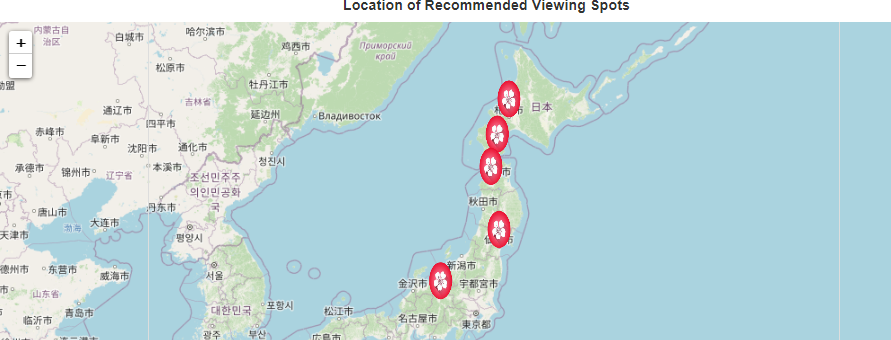
\includegraphics[]{images/RecommendedViewingSpots.png}
\caption{\small{From South to North: Matsumoto Castle, Mikamine Park, Hirosaki Castle, Goryokaku Fort, Maruyama Park and Hokkaido Shrine}}
\end{figure}    

The recommended viewing spots are all located in the northern regions of Japan. This is not surprising due to the time of Hanami season 
we are focusing on. The cherry blossom front travels from south to north, with the start of Hanami season occurring in the southern regions
of Japan around late March and the end of the season occurring in late May in the northern regions of Japan.

    \hypertarget{clustering-train-stations-hierarchical-clustering}{%
\subsection{Clustering Train Stations : Hierarchical
Clustering}\label{clustering-train-stations-hierarchical-clustering}}

When reviewing the venues dataframe, it was found there were multiple \texttt{Train Station} and \texttt{Platform} venues,
for a single train station. An example of this is shown on Figure 2 for the Goryokaku Station near Goryokaku Fort. 

\begin{figure}[H]
  \centering
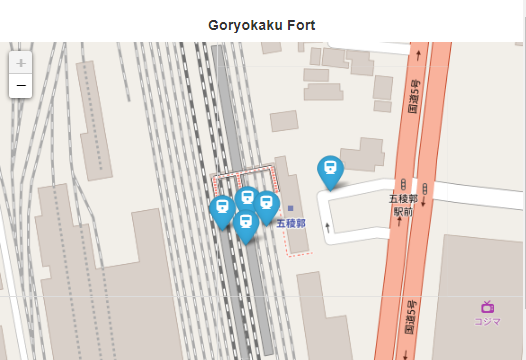
\includegraphics[]{images/TrainClusterExample.png}
\caption{Example of multiple Train Station and Platform venues around one Train Station.}
\end{figure}

We want there to be only one set of coordinates per train station. We could pick the points visually to condense into one point
per venue, but let's accomplish this through use of hierarchical clustering.

The process which was taken to determine the number of clusters for the excess coordinates 
around each train station was:

\begin{itemize}
  \tightlist
  \item All \texttt{Train\ Station} and \texttt{Platform} points were identified. 
  \item Dendograms were created for each of the recommended viewing spots. 
  \item Number of clusters was determined from the dendograms by use of a threshold line. This line was drawn from the euclidean distance of 
  0.002, which is \textasciitilde200 meters (\textasciitilde0.12 miles) from next point. 
  \item The number of times the threshold line crosses a horizontal line determines the number of clusters.
\end{itemize}

    \hypertarget{dendograms}{%
\subsubsection{Dendograms}\label{dendograms}}

\begin{figure}[H]
  \centering
  \begin{subfigure}[t]{0.45\textwidth}
    \centering
    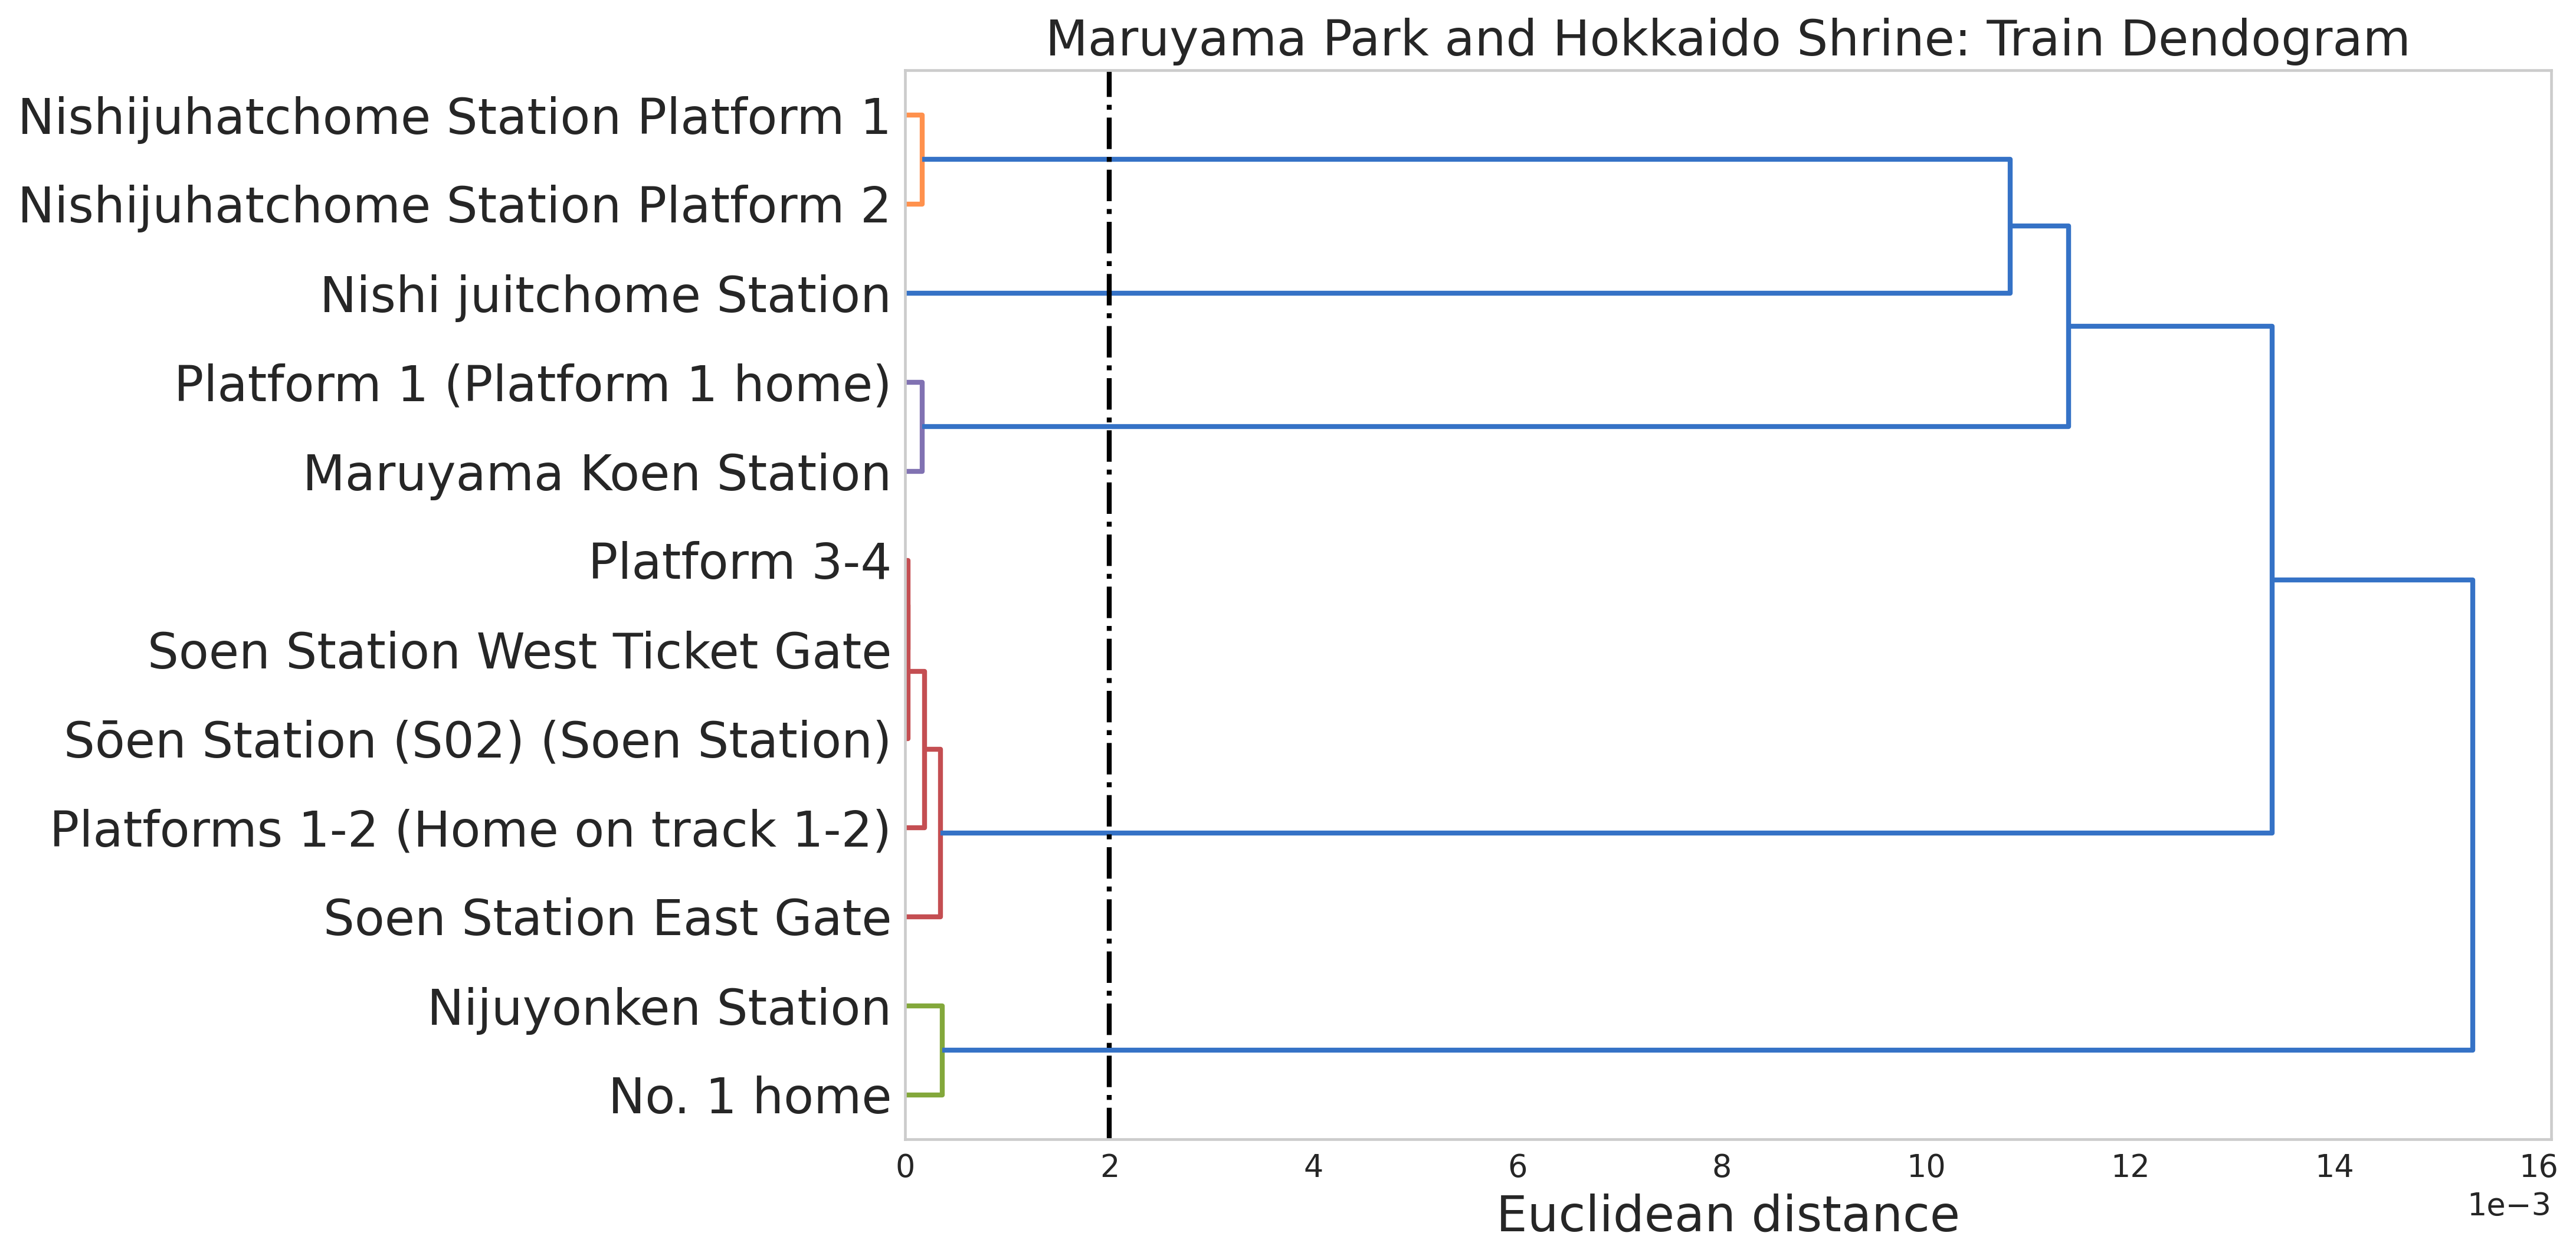
\includegraphics[width=\textwidth]{images/Maruyama Park and Hokkaido Shrine__threshold.png}
  \end{subfigure}
  \hfill
  \begin{subfigure}[t]{0.49\textwidth}
    \centering
    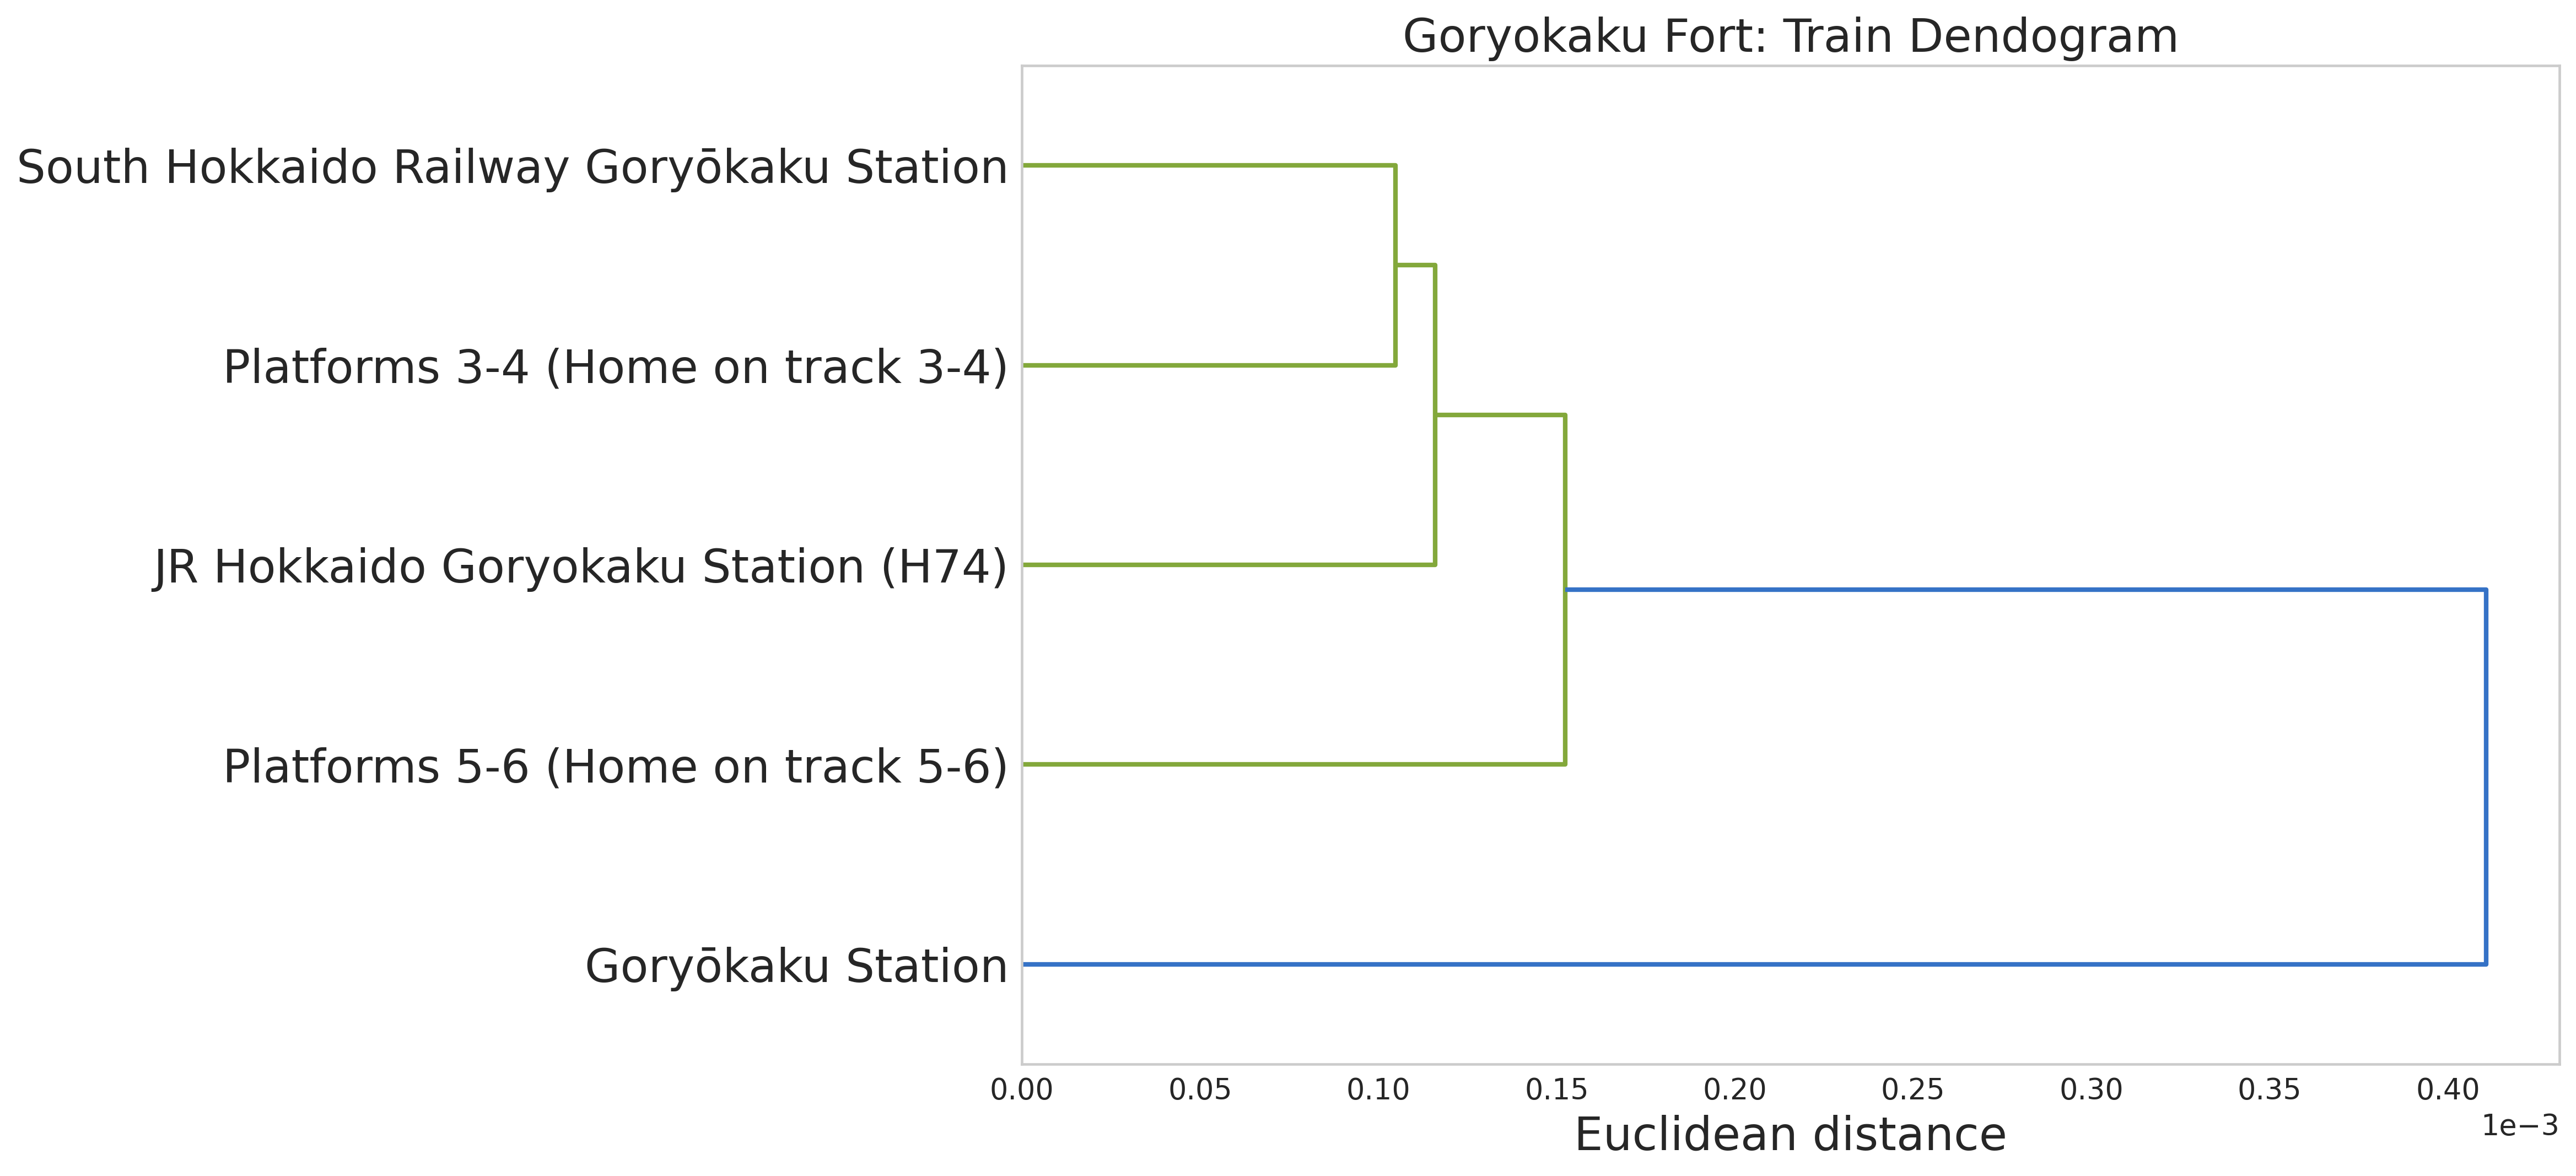
\includegraphics[width=\textwidth]{images/Goryokaku Fort__threshold.png}
  \end{subfigure}

  \vfill
  \centering
  \begin{subfigure}[c]{0.45\textwidth}
    \centering
    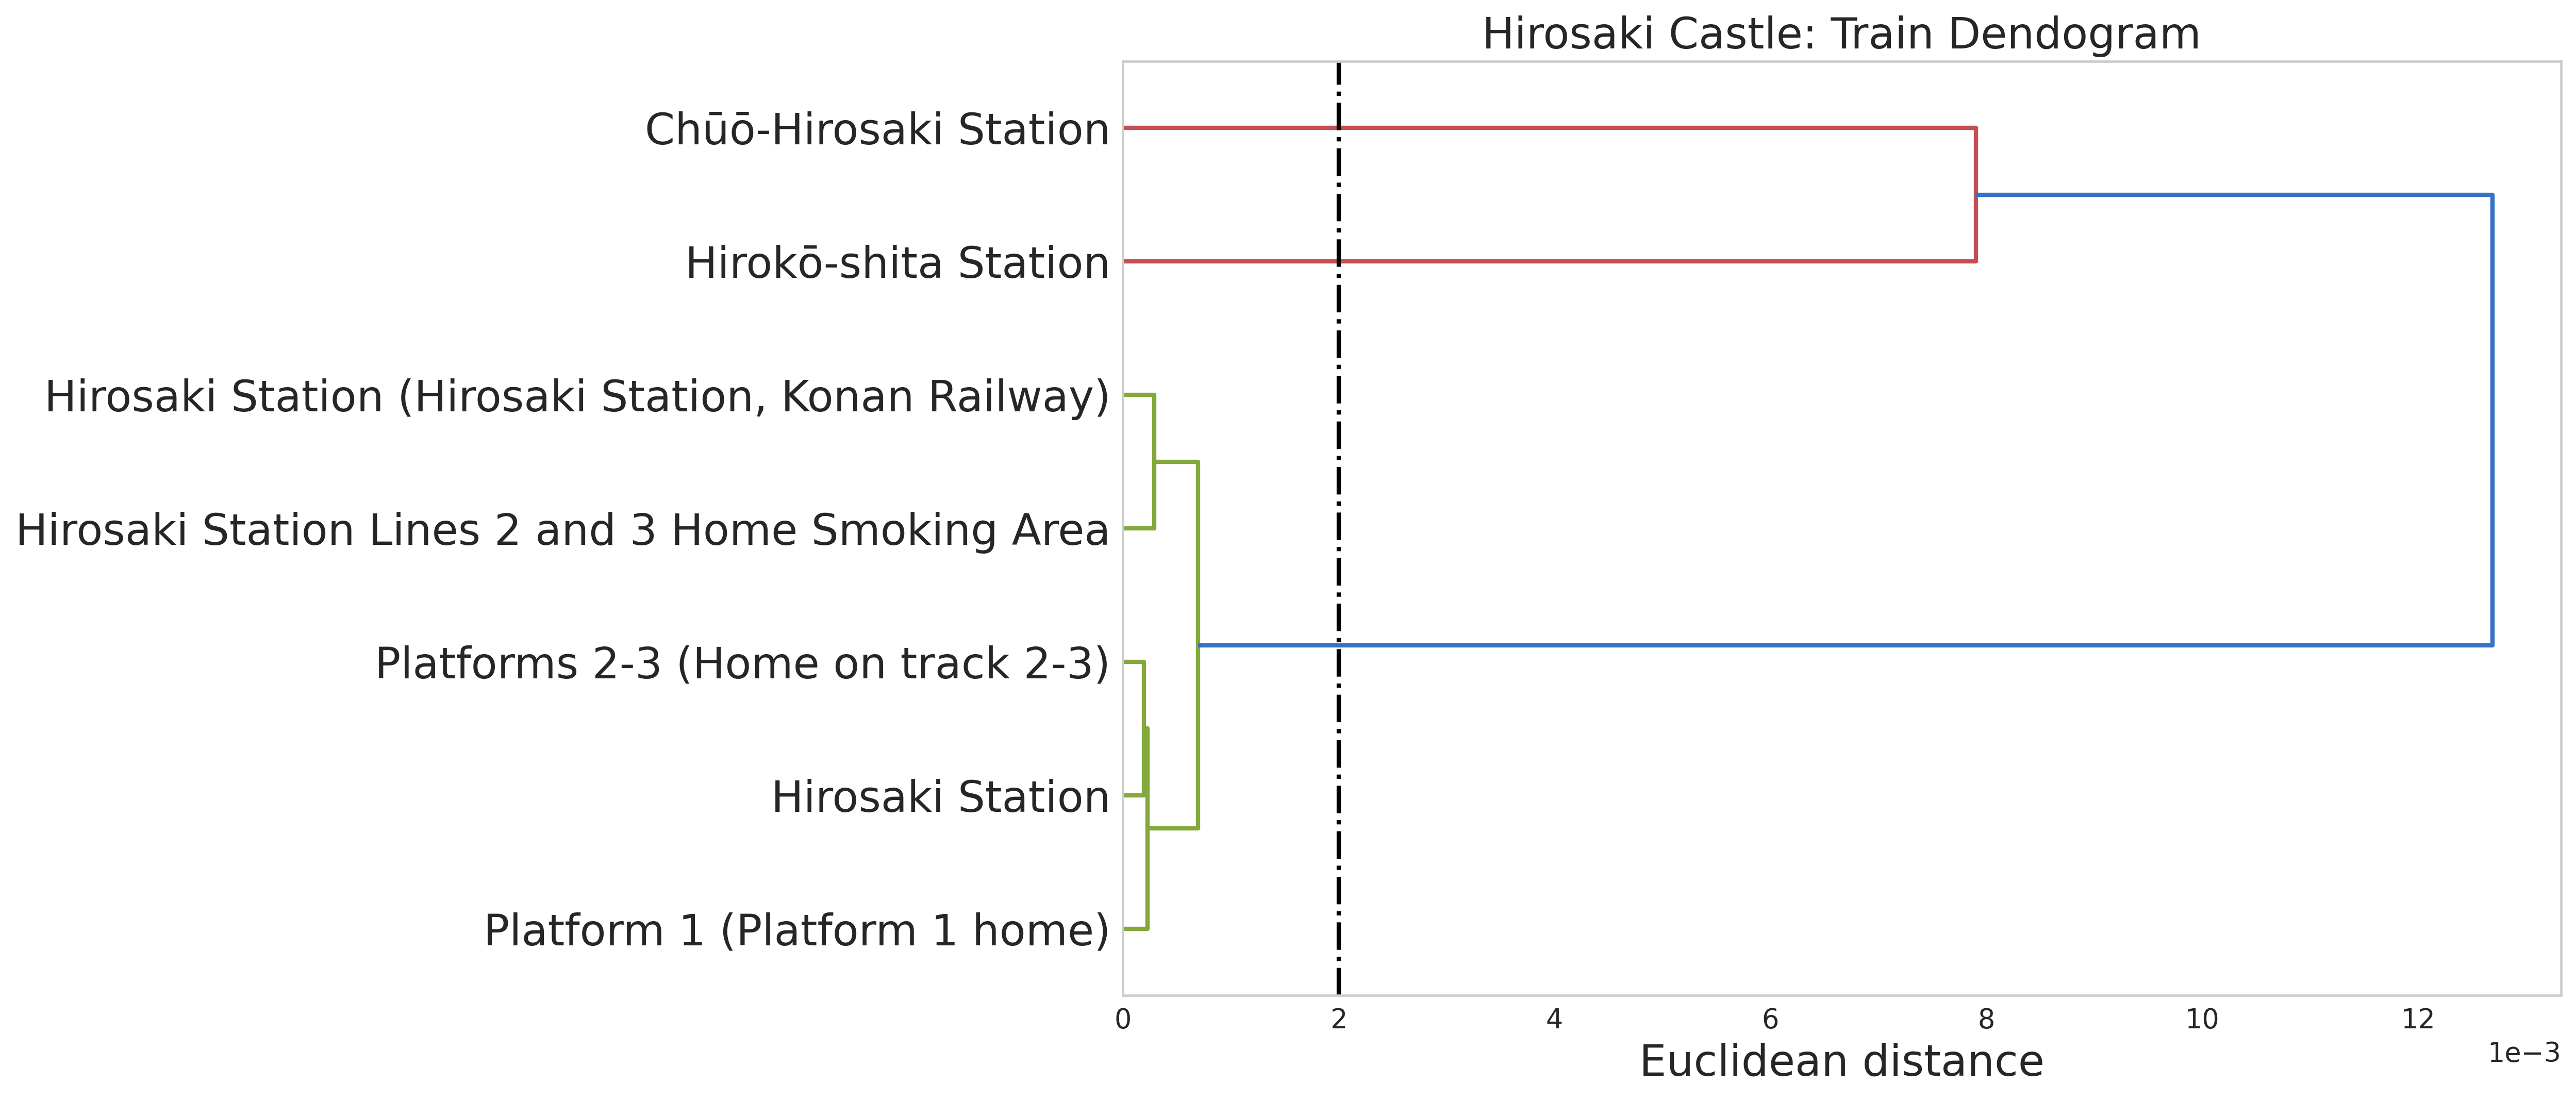
\includegraphics[width=\textwidth]{images/Hirosaki Castle__threshold.png}
  \end{subfigure}
  \hfill
  \begin{subfigure}[c]{0.4 \textwidth}
    \centering
    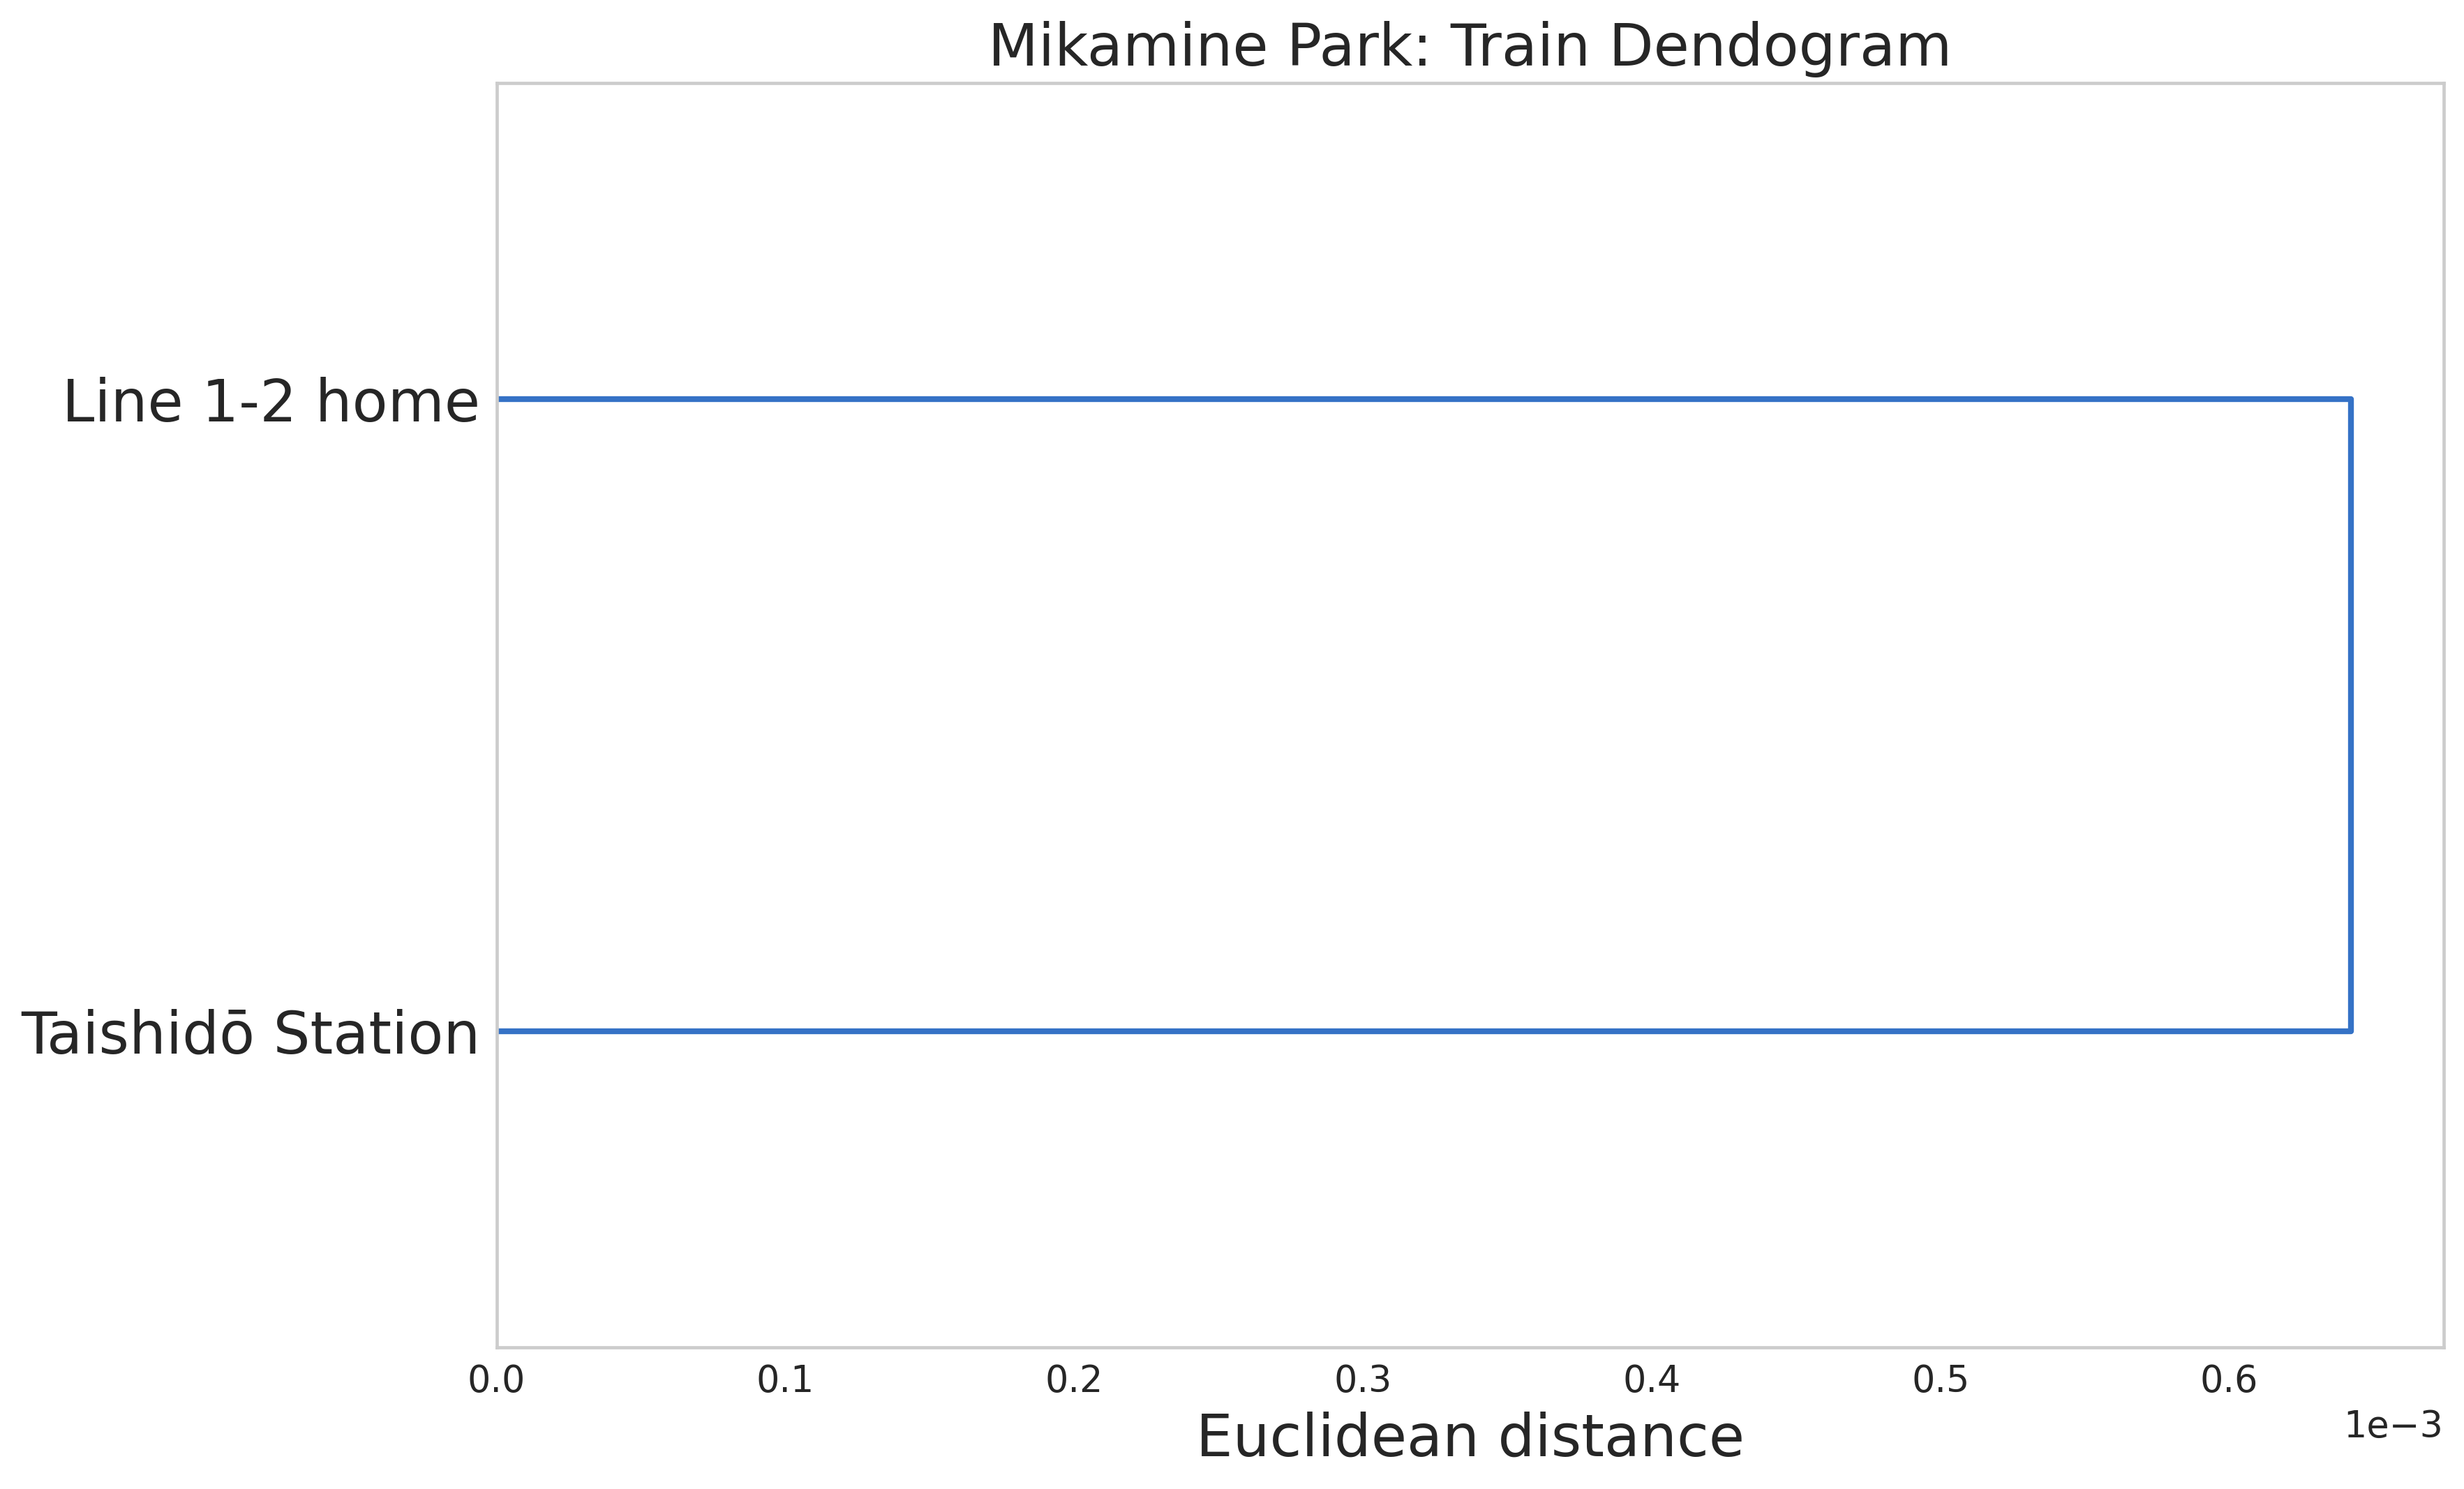
\includegraphics[width=\textwidth]{images/Mikamine Park__threshold.png}
  \end{subfigure}

  \vfill
  \begin{subfigure}[b]{0.6\textwidth}
    \centering
    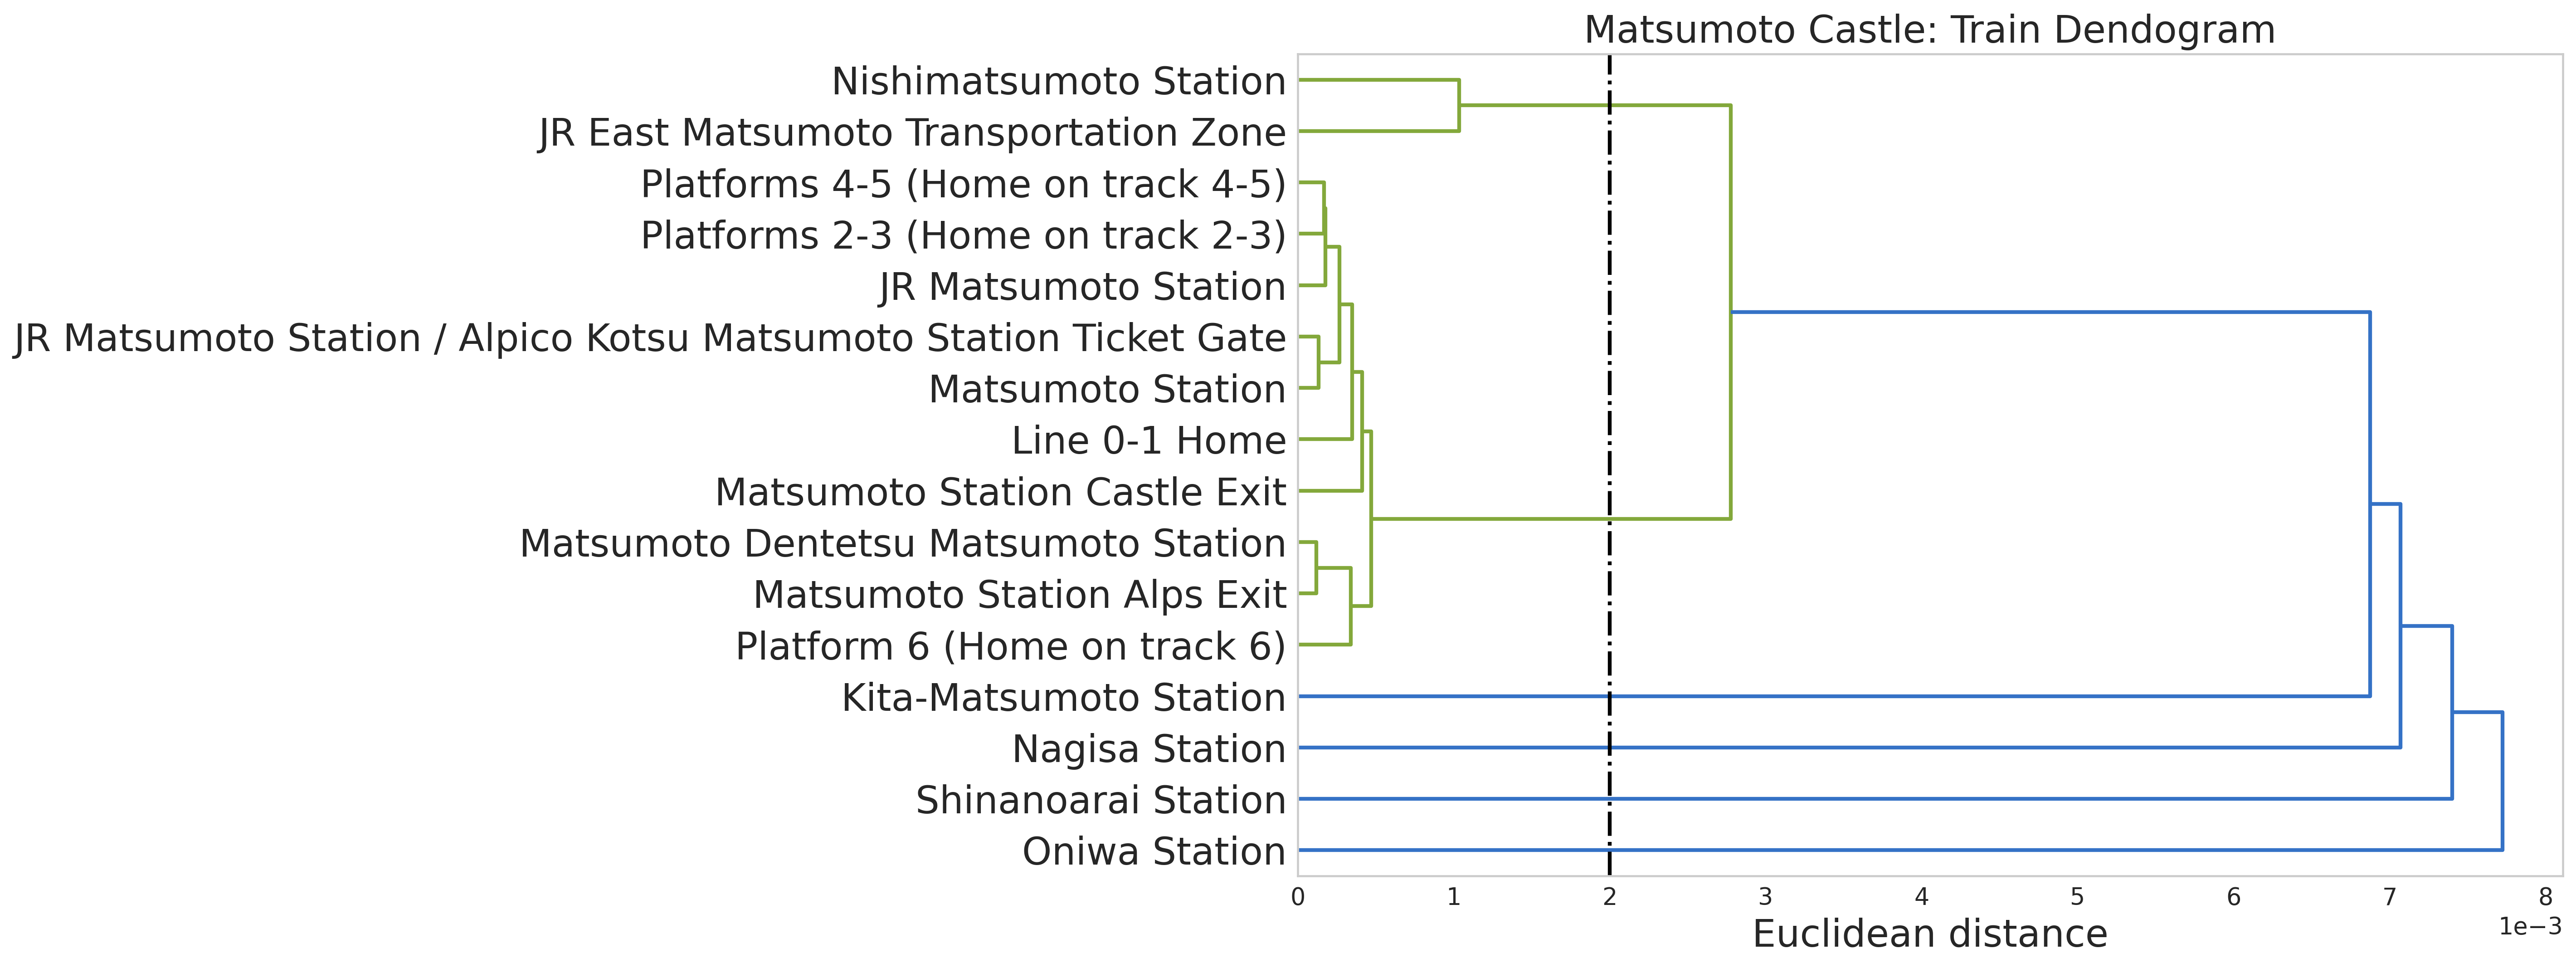
\includegraphics[width=\textwidth]{images/Matsumoto Castle__threshold.png}
  \end{subfigure}
  \caption{Dendograms for train locations around each of the Recommended Viewing Spots.}
\end{figure}

    We were looking to create clusters with a euclidean distance of at least
\texttt{0.002} (\textasciitilde{} 200meters / \textasciitilde0.12
miles). The distance between the points at \texttt{Goryokaku\ Fort} and
\texttt{Mikamine\ Park} are relatively small compared to the other three
locations. It is for this reason those points in those areas will be one
cluster.

\begin{itemize}
\tightlist
\item
  Maruyama Park and Hokkaido Shrine : 5 clusters
\item
  Goryokaku Fort : 1 cluster
\item
  Hirosaki Castle : 3 clusters
\item
  Mikamine Park : 1 cluster
\item
  Matsumoto Castle : 6 clusters
\end{itemize}

    \hypertarget{agglomerative-clustering}{%
\subsubsection{Agglomerative
Clustering}\label{agglomerative-clustering}}

With the number of clusters determined through the use of dendograms, the excess number of train station venue 
coordinates are clustered together with those in close vicinity of one another for each of the recommended 
viewing spots.

The train station and Platform venues will be plotted. Those belonging to the same
cluster are assigned the same color and label based off their cluster.

\begin{figure}[H]
  \centering
  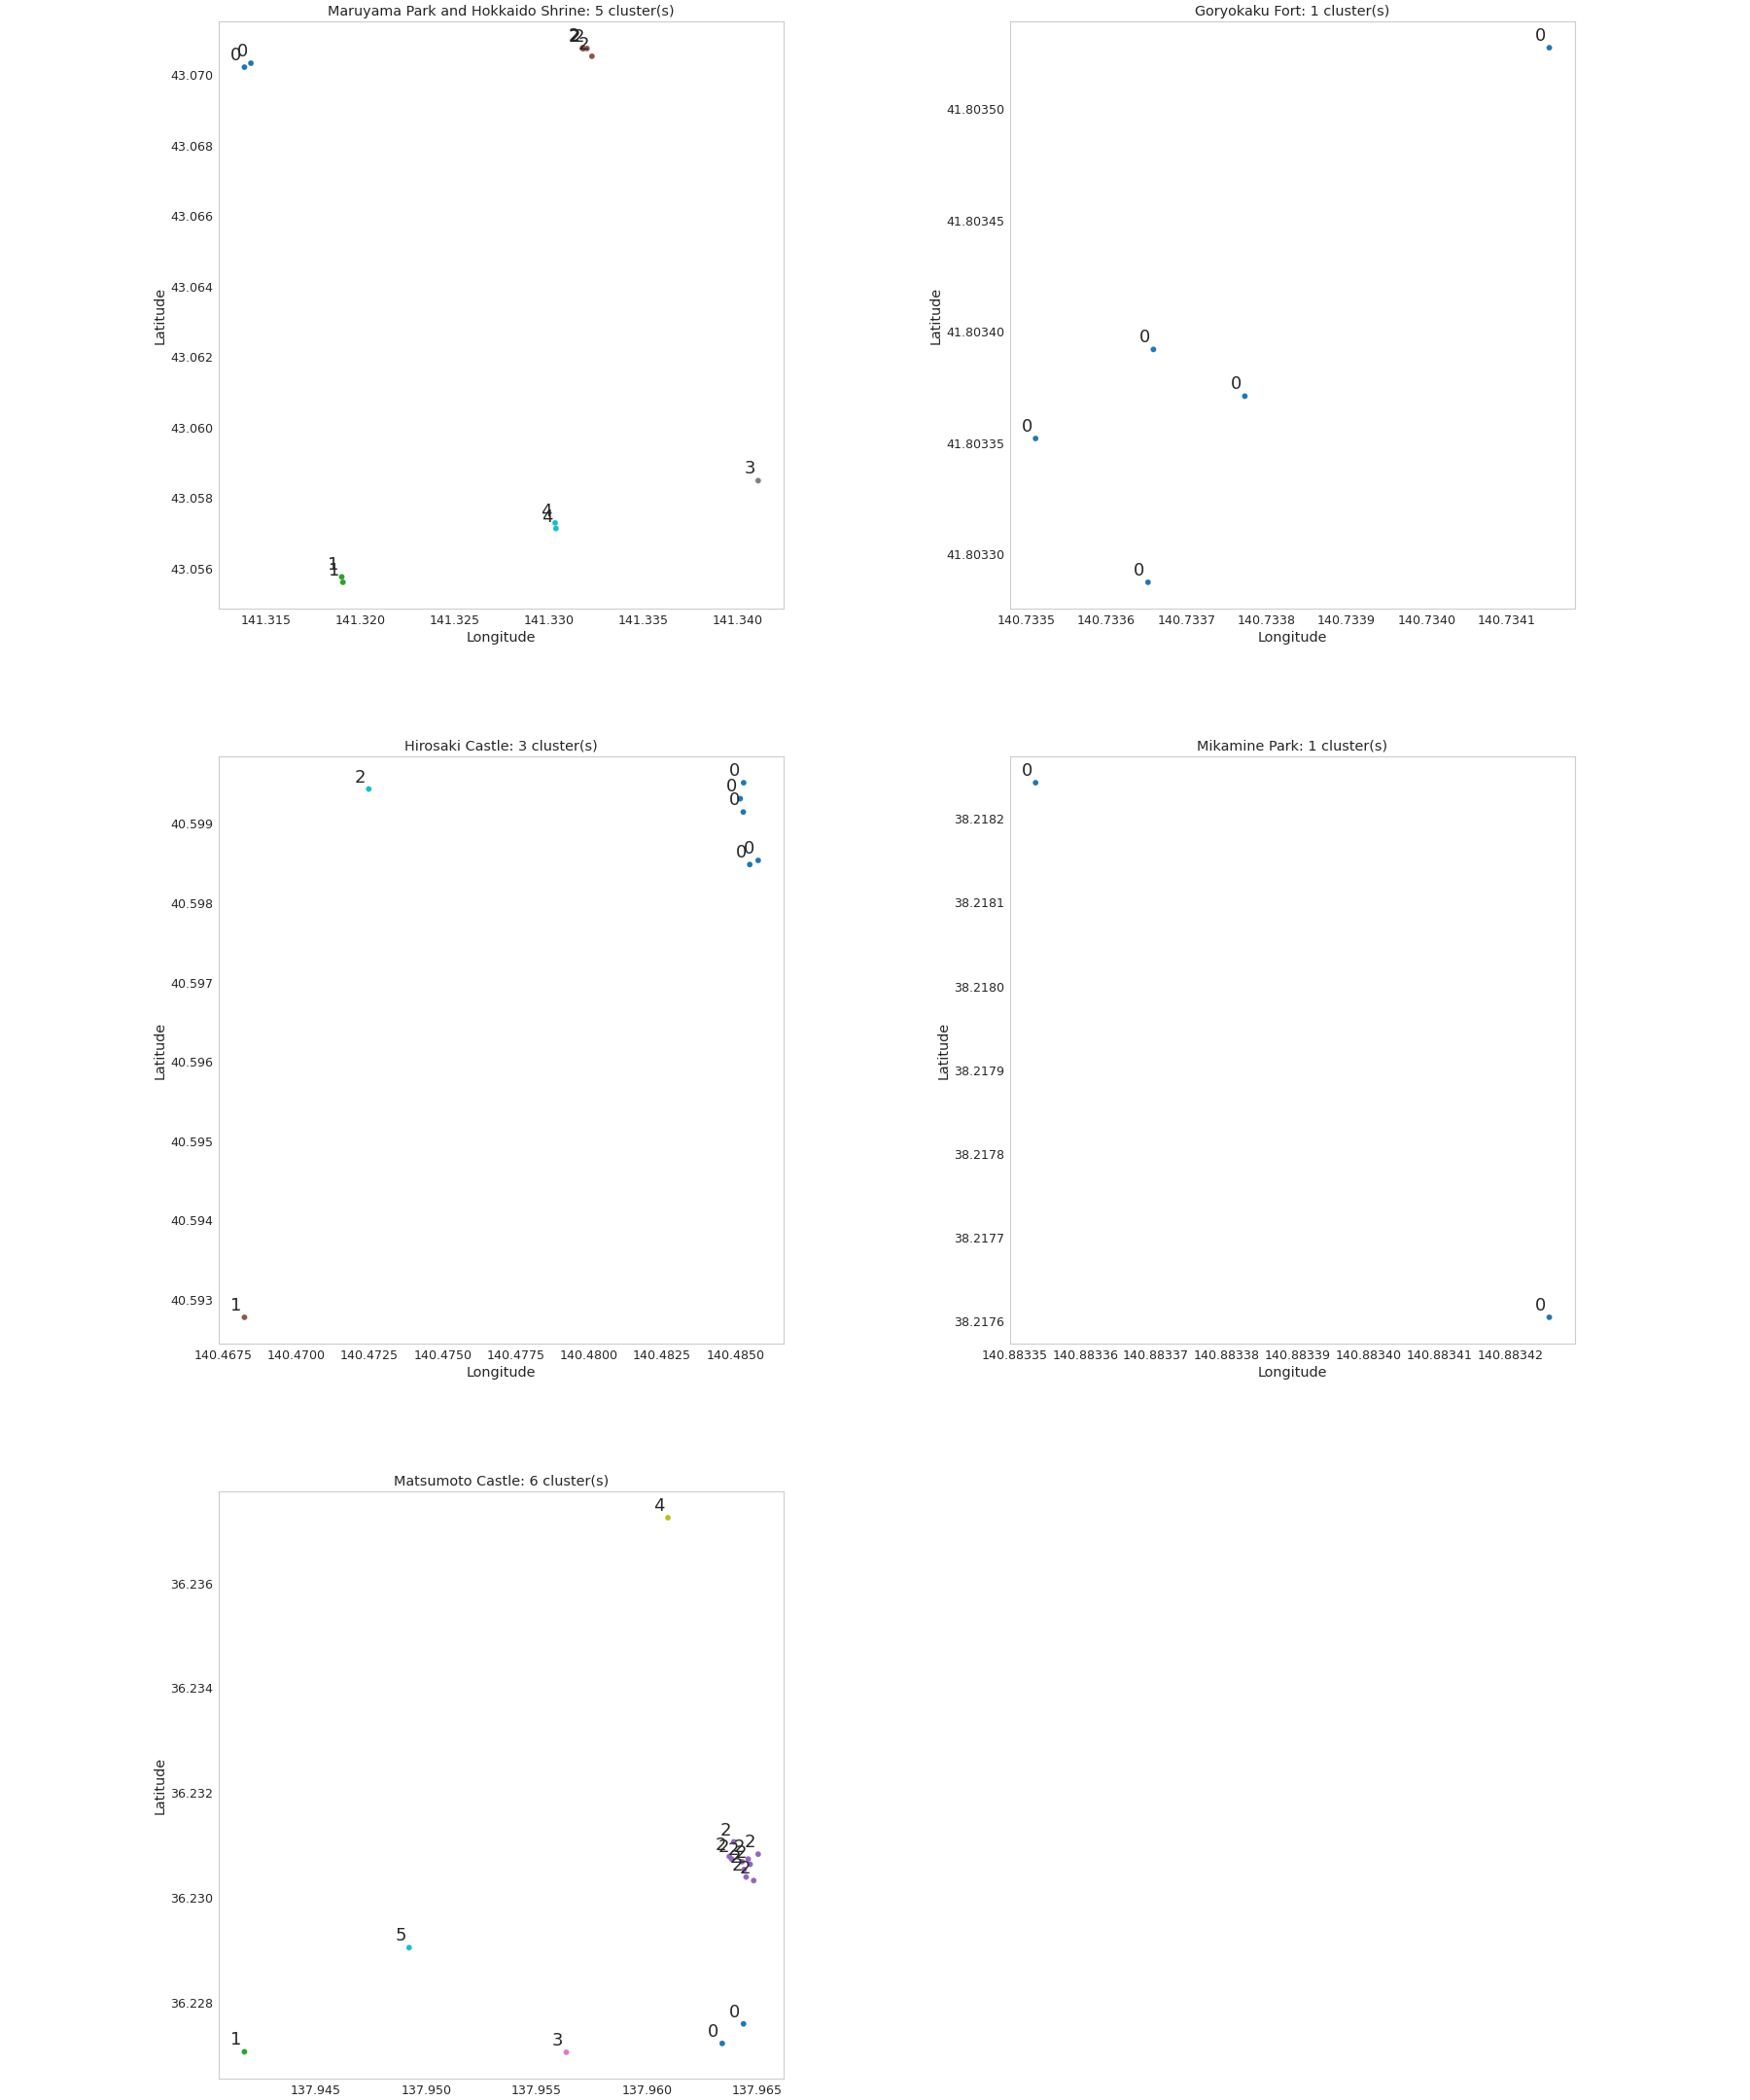
\includegraphics[]{images/Train_Clusters.png}
  \caption{Agglomerative Clustering: Train Clusters for each of the recommended viewing spots.}
 \end{figure}
    
These clusters were used to reduce the number of excess train station and platform points around 
a single train station venue.
    
    \begin{Verbatim}[commandchars=\\\{\}]
Original Number of Train Stations: 42.
Current Number of Train Stations: 16.
    \end{Verbatim}

    \hypertarget{summary-of-clustering}{%
\subsubsection{Summary of Clustering}\label{summary-of-clustering}}

42 \texttt{Train\ Station} and \texttt{Platform} points were reduced to 16
\texttt{Train\ Station} points across the 5 recommended viewing spot
areas.

With all the extra train station coordinates reduced around each of the
viewing spots, the \texttt{venues} dataframe was updated to with the new
train station information while removing the old information.

    \hypertarget{plot-venues-around-recommended-viewing-spots}{%
\subsection{Plot venues around Recommended Viewing Spots}\label{plot-venues-around-recommended-viewing-spots}}

Plotting all the venues around each the viewing spots. Restaurants will be indicated 
by a cutlery icon, while train stations will be indicated by a train icon. On each map a circle
with a radius of 1.25 miles is centered on the recommended viewing spot.

\begin{figure}[H]
  \centering
  \begin{subfigure}[t]{0.45\textwidth}
    \centering
    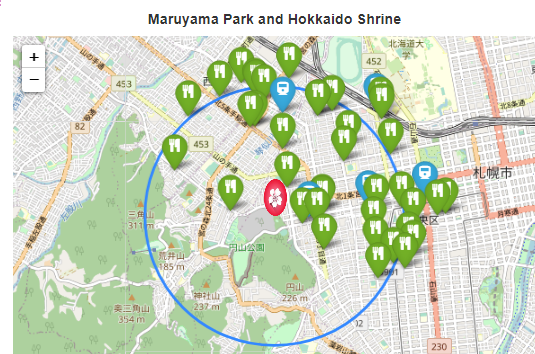
\includegraphics[width=\textwidth]{images/Maruyama Park and Hokkaido Shrine_venues.png}
  \end{subfigure}
  \hfill
  \begin{subfigure}[t]{0.45\textwidth}
    \centering
    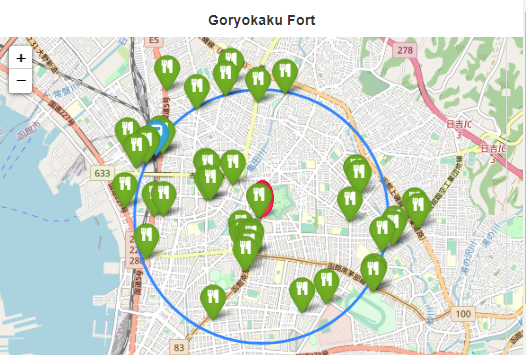
\includegraphics[width=\textwidth]{images/Goryokaku Fort_venues.png}
  \end{subfigure}

  \vfill
  \centering
  \begin{subfigure}[c]{0.45\textwidth}
    \centering
    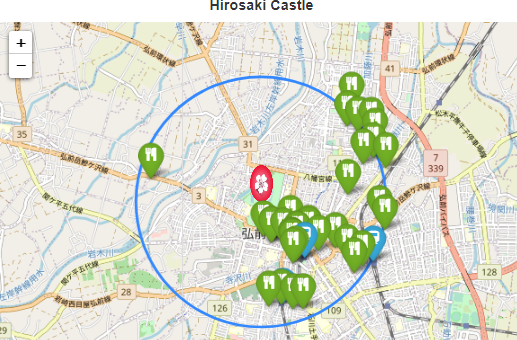
\includegraphics[width=\textwidth]{images/Hirosaki Castle_venues.png}
  \end{subfigure}
  \hfill
  \begin{subfigure}[c]{0.45\textwidth}
    \centering
    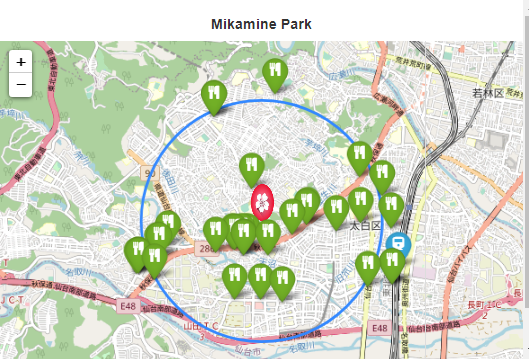
\includegraphics[width=\textwidth]{images/Mikamine Park_venues.png}
  \end{subfigure}

  \vfill
  \begin{subfigure}[b]{0.45\textwidth}
    \centering
    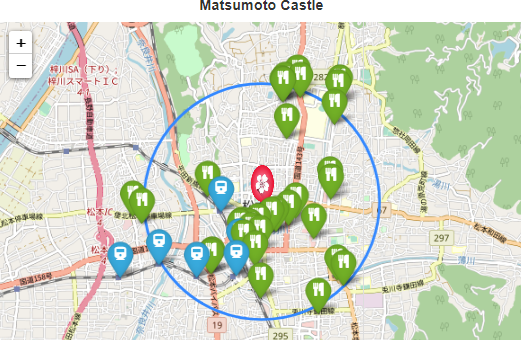
\includegraphics[width=\textwidth]{images/Matsumoto Castle_venues.png}
  \end{subfigure}
  \caption{Dendograms for train locations around each of the Recommended Viewing Spots.}
\end{figure}
        
    \hypertarget{comparing-the-recommended-viewing-spots}{%
\subsection{Comparing the Recommended Viewing
Spots}\label{comparing-the-recommended-viewing-spots}}

    Let's group rows by Viewing Spot and by taking the mean of the frequency
of occurrence of each category

\begin{table}[h]
\centering
\small
\caption{Frequency of Occurrence of each Category}
\begin{tabular}{lcc}
\toprule
VIEWING\_SPOT                      &  Ramen Restaurant &  Train Station \\
\midrule
                   Goryokaku Fort & 0.976744          & 0.023256       \\
                  Hirosaki Castle & 0.923077          & 0.076923       \\
Maruyama Park and Hokkaido Shrine & 0.883721          & 0.116279       \\
                 Matsumoto Castle & 0.850000          & 0.150000       \\
                    Mikamine Park & 0.970588          & 0.029412       \\
\bottomrule
\end{tabular}
\end{table}

        
    Not very informative due to only two types of venues.

Let's look at how each of the viewing spots compare to one another in
regards to Ramen Restaurants and Train Stations.

We will do this through the use of a bar charts.

First, let's see how the number of Ramen Restaurants and Train Stations
compare.

\begin{figure}[H]
  \centering
  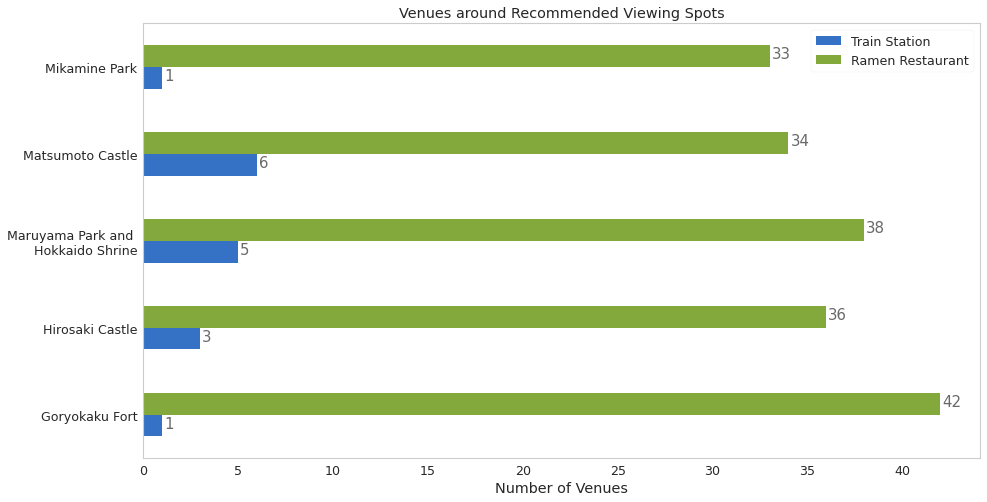
\includegraphics[]{images/Venue_Count.png}
  \caption{}
\end{figure}

    
    Next, let's see the average distance to Ramen Restaurants and Train
Stations.

\begin{figure}[H]
  \centering
  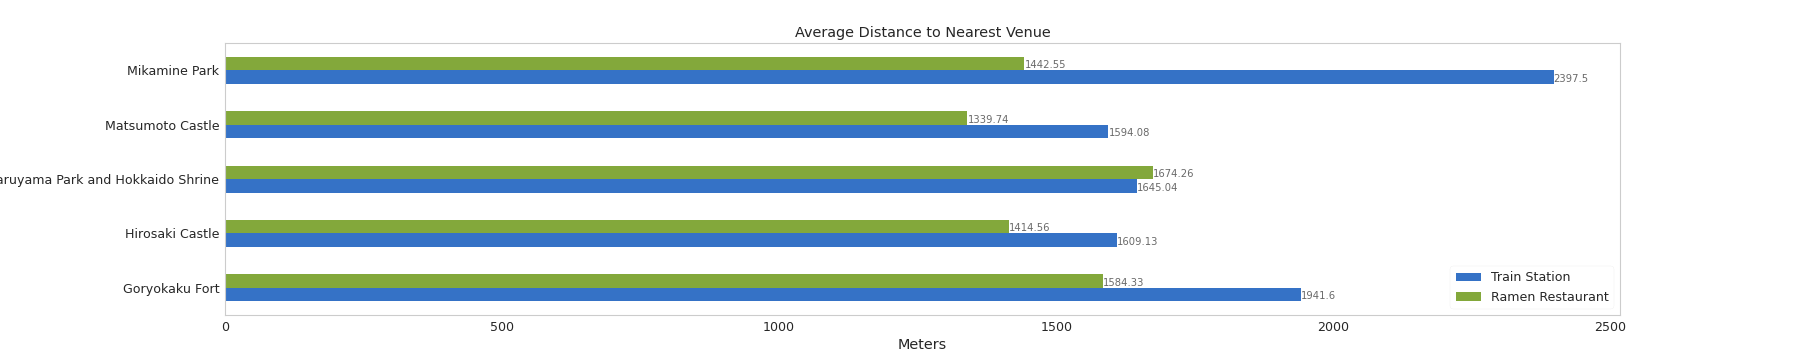
\includegraphics[]{images/Average_Venue_Distance.png}
  \caption{}
\end{figure}
    
    \hypertarget{results-and-discussion}{%
\section{Results and Discussion}}\label{results-and-discussion}

    From the many Hanami spots across Japan, five Hanami spots (Mikamine
Park, Matsumoto Castle, Maruyama Park and Hokkaido Shrine, Hirosaki
Castle, and Goryokaku Fort) were selected based off average cherry
blossoming time occurring between April 15th - May 15th and based off
recommendations from
\url{https://www.japan-guide.com/e/e2011_where.html}. Our analysis of
these five recommended Hanami spots showed there are a quite a number of
Ramen Shops/Restaurants and at least one train station around each
location.

Now, how can we determine which of the five recommended Hanami Spots
should be selected as the \emph{best}. The criteria that will be used are:
1) Ramen shops located close to the recommended Hanami spots and 2)
Proximity to a train station.

\begin{enumerate}
\def\labelenumi{\arabic{enumi})}
\item
  Ramen Shops

  We can quickly compare the number of Ramen Shops between each of the
  five Hanami Spots by looking at Figure 6. Based off number of Ramen
  shops alone, Goryokaku Fort is the \emph{best} of the recommended Hanami
  Spots with 42 Ramen Shops and Mikamine Park is the \emph{worst} with only
  33 Ramen Shops within a 1.25 mile radius. 
  
  Furthermore looking at Figure 7, the \emph{best} Hanami Spot would be Matsumoto Castle with a Ramen Shop
  located within an average distance of 1340 meters
  (\textasciitilde0.83 miles) and the \emph{worst} location would be
  Maruyama Park and Hokkaido Shrine with a Ramen Shop located within an
  average distance of 1674 meters (\textasciitilde1.04
  miles).
\item
  Train Stations

  Chart B indicates Matsumoto Castle would be the \emph{best} location to enjoy
  Hanami and grab a train due to the average distance to a train station
  is 1594 meters with six train stations in the area.
  While Mikamine Park is the \emph{worst} with an average distance of
  2398 meters with only the one train station in the
  area.
\end{enumerate}

Another criterion to select the \emph{best} Hanami spot is to use the
rating system found at \url{https://www.japan-guide.com/e/e2011_where.html}. 
The rating for each of the recommended Hanami spots were also scraped from 
the site and can be found within the \texttt{viewingSpot\_df} dataset. The 
ratings range from 1 to 3 where the numbers represent the following:

\begin{enumerate}
\def\labelenumi{\arabic{enumi})}
\item
  Recommended
\item
  Highly Recommended
\item
  Best of Japan
\end{enumerate}


\begin{table}[h]
  \tiny
  \centering
  \caption{Recommended Viewing Spots Sorted by Rating}
  \begin{tabular}{llllllcr}
  \toprule
  VIEWING\_SPOT                     & CITY      & PREFECTURE & REGION   &  LATITUDE &  LONGITUDE & RATING  & RATING\_DESCRIPTION \\
  \midrule
                    Hirosaki Castle &  Hirosaki &   Aomori   &   Tohoku & 40.607452 & 140.464180 &  3      &      Best of Japan \\
                     Goryokaku Fort &  Hakodate & Hokkaido   & Hokkaido & 41.794670 & 140.754020 &  2      & Highly Recommended \\
                   Matsumoto Castle & Matsumoto &   Nagano   &    Chubu & 36.238653 & 137.968867 &  2      & Highly Recommended \\
  Maruyama Park and Hokkaido Shrine &   Sapporo & Hokkaido   & Hokkaido & 43.055745 & 141.312607 &  1      &        Recommended \\
                      Mikamine Park &    Sendai &   Miyagi   &   Tohoku & 38.224822 & 140.857414 &  1      &        Recommended \\
  \bottomrule
  \end{tabular}
  \end{table}
  
        
    Based off the rating system, Hirosaki Castle is the best Hanami Spot
from the bunch to visit. Not only is it considered a \emph{Best of Japan}
location, it has 36 Ramen Shops within an average distance of
1415 meters (\textasciitilde{} 0.88 miles) and 3 Trains
stations within an average distance of \textasciitilde1609 meters
(\textasciitilde{} 1.0 mile).

    \hypertarget{conclusion}{%
\section{Conclusion}}\label{conclusion}

    In this project, we identified some of the best locations in Japan in
which to enjoy both Hanami and Ramen from April 15th to May 15th. We
found recommended Hanami spots which could be traveled to easily based on the proximity
of train stations and also found that each of the spots have a good variety
of choices for Ramen.

We also were able to cluster multiple coordinates together for
a single train station based off their proximity to one another through the 
use of Hierarchical clustering. The ability to quickly compare the number of
venues around each of the recommended Hanami Spots was accomplished
through the use of bar charts.

Overall, there are many different locations a person can visit to enjoy
springtime and the cherry blossoms in Japan. The biggest factor to keep
in mind is the when. With cherry blossoms lasting a short time span and
the cherry blossom front traveling from south to north, a person needs
to keep the time of spring season in mind when planning a trip to Japan to
experience the tradition of Hanami.


    % Add a bibliography block to the postdoc
    
    
    
\end{document}
